\documentclass[bachelor,ngerman,english]{GAUBM}

\usepackage{setspace}  %% Zur Setzung des Zeilenabstandes
\usepackage{blindtext}
\usepackage{float}
\usepackage{svg}
\usepackage{babel}     %% Sprachen-Unterstuetzung
\usepackage{calc}      %% ermoeglicht Rechnen mit Laengen und Zaehlern
\usepackage[T1]{fontenc}       %% Unterstutzung von Umlauten etc.
\usepackage[utf8]{inputenc}  %% 
%% in aktuellem Linux & MacOS X wird standardmaessig UTF8 kodiert!
%\usepackage[utf8]{inputenc}    %% Wenn latin1 nicht geht ...
\usepackage{amsmath,amssymb} %% zusaetzliche Mathe-Symbole
\usepackage{lmodern} %% type1-taugliche CM-Schrift als Variante zur
                     %% "normalen" EC-Schrift
%% Paket fuer bibtex-Datenbanken
\usepackage[comma,numbers,sort&compress]{natbib}
\bibliographystyle{datenbank}
% \bibliographystyle{plainnat}

\newcommand{\tabheadfont}[1]{\textbf{#1}} %% Tabellenkopf in Fett
\usepackage{booktabs}                      %% Befehle fuer besseres Tabellenlayout
\usepackage{longtable}                     %% umbrechbare Tabellen
\usepackage{array}                         %% zusaetzliche Spaltenoptionen

%% umfangreiche Pakete fuer Symbole wie \micro, \ohm, \degree, \celsius etc.
\usepackage{textcomp,gensymb}
%\usepackage{SIunits} %% Korrektes Setzen von Einheiten
\usepackage{units}   %% Variante fuer Einheiten
\usepackage[pdfstartview=FitH,      % Oeffnen mit fit width
            breaklinks=true,        % Umbrueche in Links, nur bei pdflatex default
            bookmarksopen=true,     % aufgeklappte Bookmarks
            bookmarksnumbered=true  % Kapitelnummerierung in bookmarks
            ]{hyperref}

\usepackage{amsmath}
\usepackage{scrhack}
\usepackage[table]{xcolor}

\newcolumntype{L}[1]{>{\raggedright\arraybackslash}p{#1}}
\newcolumntype{C}[1]{>{\centering\arraybackslash}p{#1}}
\newcolumntype{R}[1]{>{\raggedleft\arraybackslash}p{#1}}
\newcolumntype{?}{!{\vrule width .1mm}}
\newcolumntype{V}{!{\vrule width .3mm}}
%\documentclass[11pt, a4paper, headsepline, footsepline]{scrbook}

%

\setlength{\oddsidemargin}{0cm}
\setlength{\evensidemargin}{0cm}
\setlength{\topmargin}{-1cm}
\setlength{\textheight}{23cm}
\setlength{\textwidth}{16cm}

\pagestyle{headings}

\renewcommand{\sectfont}{\bfseries\rmfamily}
\renewcommand{\floatpagefraction}{0.7}
\renewcommand{\textfraction}{0.1}

% abbreviations added, A.Quadt, 07.09.2010
\newcommand{\ttbar}         {\mbox{$t\bar{t}$}\xspace}
\newcommand{\ttZ}           {\mbox{$t\bar{t}Z$}\xspace}
\newcommand{\ttW}           {\mbox{$t\bar{t}W$}\xspace}
\newcommand{\ttH}           {\mbox{$t\bar{t}H$}\xspace}
\newcommand{\ttHWW}         {\mbox{$t\bar{t}(H\rightarrow WW^*)$}\xspace}
\newcommand{\HWW}           {\mbox{$H\rightarrow WW^*$}\xspace}
\newcommand{\Hbb}           {\mbox{$H\rightarrow bb$}\xspace}
\newcommand{\spanet}        {\texttt{SPA-Net}\xspace}
\newcommand{\spanets}       {\texttt{SPA-Net}'s\xspace}

\newcommand{\tquark}   	{top quark\xspace}
\newcommand{\tquarks}   {top quarks\xspace}
\newcommand{\bquark}   	{bottom quark\xspace}
\newcommand{\bquarks}   {bottom quarks\xspace}
\newcommand{\zboson}   	{$Z$ boson\xspace}
\newcommand{\zbosons}  	{$Z$ bosons\xspace}
\newcommand{\wboson}   	{$W$ boson\xspace}
\newcommand{\wbosons}  	{$W$ bosons\xspace}
\newcommand{\zwboson}   {$Z$/$W$ boson\xspace}
\newcommand{\Hboson}  	{Higgs boson\xspace}
\newcommand{\Hbosons}  	{Higgs bosons\xspace}

\newcommand{\dzero}      {D\O\xspace}
\newcommand{\cdf}        {CDF\xspace}
\newcommand{\qqbar}      {\mbox{$q\bar{q}$}}
\newcommand{\uubar}      {\mbox{$u\bar{u}$}}
\newcommand{\ddbar}      {\mbox{$d\bar{d}$}}
\newcommand{\ccbar}      {\mbox{$c\bar{c}$}}
\newcommand{\ssbar}      {\mbox{$s\bar{s}$}}
\newcommand{\bbbar}      {\mbox{$b\bar{b}$}}
\newcommand{\wjets}      {\mbox{$W + 4\; jets$}}
\newcommand{\pttbar}     {\mbox{$p_{t\bar{t}}$}}
\newcommand{\pwjets}     {\mbox{$p_{W +4 \; jets}$}}
\newcommand{\ljets}      {\mbox{$\ell + \; jets$}}
\newcommand{\ejets}      {\mbox{$e + \; jets$}}
\newcommand{\mujets}     {\mbox{$\mu + \; jets$}}
%
%
\newcommand{\fermilab}  {{F{\textsc{ermilab}}}\xspace}
\newcommand{\tevatron}  {{T{\textsc{evatron}}}\xspace}
\newcommand{\opal}      {{O{\textsc{pal}}}\xspace}
\newcommand{\cern}      {{C{\textsc{ern}}}\xspace}
\newcommand{\fnal}      {{F{\textsc{nal}}}\xspace}
\newcommand{\atlas}     {{A{\textsc{tlas}}}\xspace}
\newcommand{\lhc}       {{L{\textsc{hc}}}\xspace}
\newcommand{\lhcb}      {{L{\textsc{hc}}}{\scriptsize{b}}\xspace}
\newcommand{\lep}       {{L{\textsc{ep}}}\xspace}
\newcommand{\slc}       {{S{\textsc{lc}}}\xspace}
\newcommand{\pep}       {{P{\textsc{ep}}}\xspace}
\newcommand{\petra}     {{P{\textsc{etra}}}\xspace}
\newcommand{\hera}      {{H{\textsc{era}}}\xspace}
\newcommand{\lepaleph}  {{A{\textsc{leph}}}\xspace}
\newcommand{\delphi}    {{D{\textsc{elphi}}}\xspace}
\newcommand{\leplthree} {{L{\textsc{3}}}\xspace}
\newcommand{\lepopal}   {{O{\textsc{pal}}}\xspace}
\newcommand{\doris}     {{D{\textsc{oris}}}\xspace}
\newcommand{\isr}       {{I{\textsc{sr}}}\xspace}
\newcommand{\desy}      {{D{\textsc{esy}}}\xspace}
\newcommand{\kek}       {{K{\textsc{ek}}}\xspace}
\newcommand{\slac}      {{S{\textsc{lac}}}\xspace}
\newcommand{\tristan}   {{T{\textsc{ristan}}}\xspace}
\newcommand{\cms}       {{C{\textsc{ms}}}\xspace}
\newcommand{\alice}     {{A{\textsc{lice}}}\xspace}
\newcommand{\zeus}      {{Z{\textsc{eus}}}\xspace}
\newcommand{\hone}      {{H{\textsc{1}}}\xspace}
\newcommand{\minuit}    {{M{\textsc{inuit}}}\xspace}
\newcommand{\herwig}    {{H\textsc{erwig}}\xspace}
\newcommand{\acermc}    {{A\textsc{cerMC}}\xspace}
\newcommand{\evtgen}    {{E\textsc{vtgen}}\xspace}
\newcommand{\mcfm}      {{M\textsc{cfm}}\xspace}
\newcommand{\mcatnlo}   {{M\textsc{c@nlo}}\xspace}
\newcommand{\sherpa}    {{S\textsc{herpa}}\xspace}
\newcommand{\jimmy}     {{J\textsc{immy}}\xspace}
\newcommand{\cteq}      {{C\textsc{teq}}\xspace}
\newcommand{\pythia}    {{P\textsc{ythia}}\xspace}
\newcommand{\jetnet}    {{J\textsc{etnet}}\xspace}
\newcommand{\isajet}    {{I\textsc{sajet}}\xspace}
\newcommand{\jetset}    {{J\textsc{etset}}\xspace}
\newcommand{\vecbos}    {{V\textsc{ecbos}}\xspace}
\newcommand{\alpgen}    {{A\textsc{lpgen}}\xspace}
\newcommand{\vegas}     {{V\textsc{egas}}\xspace}
\newcommand{\gnu}       {{G\textsc{nu}}\xspace}
\newcommand{\onetop}    {{O\textsc{neTop}}\xspace}
\newcommand{\ztop}      {{Z\textsc{Top}}\xspace}
\newcommand{\toprex}    {{T\textsc{opRex}}\xspace}
\newcommand{\singletop} {{S\textsc{ingleTop}}\xspace}
\newcommand{\madgraph}  {{M\textsc{adgraph}}\xspace}
\newcommand{\madevent}  {{M\textsc{adevent}}\xspace}
\newcommand{\comphep}   {{C\textsc{omphep}}\xspace}
\newcommand{\qq}        {{Q\textsc{q}}\xspace}
\newcommand{\tauola}    {{T\textsc{auola}}\xspace}
\newcommand{\geant}     {{G\textsc{eant}}\xspace}
\newcommand{\GEANT}     {{G\textsc{eant}}\xspace}
\newcommand{\amegic}    {{A\textsc{megic++}}\xspace}

\newcommand{\met}       {\mbox{$\not\!\!E_T$}\xspace}
\newcommand{\metcal}    {\mbox{$\not\!\!E_{Tcal}$}\xspace}
\newcommand{\MET}       {$\not\!\!E_T$}
\newcommand{\lowmet}    {low-\mbox{$\not\!\!E_T$}-QCD\xspace}
\newcommand{\lumi}      {$\mathcal{L}$\xspace}
\newcommand{\intlumi}   {$\int\mathcal{L}\,\mathrm{d}t$\xspace}

\newcommand{\runi}      {Run~I\xspace}
\newcommand{\runii}     {Run~II\xspace}

%\newcommand{\dzero}      {D\O}
%\newcommand{\uubar}      {\mbox{$u\bar{u}$}}
%\newcommand{\ddbar}      {\mbox{$d\bar{d}$}}
%\newcommand{\ccbar}      {\mbox{$c\bar{c}$}}
%\newcommand{\ssbar}      {\mbox{$s\bar{s}$}}
%\newcommand{\ttbar}      {\mbox{$t\bar{t}$}}
%\newcommand{\bbbar}      {\mbox{$b\bar{b}$}}
%\newcommand{\wjets}      {\mbox{$W + 4\; jets$}}
%\newcommand{\pttbar}     {\mbox{$p_{t\bar{t}}$}}
%\newcommand{\pwjets}     {\mbox{$p_{W +4 \; jets}$}}
%\newcommand{\ljets}      {\mbox{$l + \; jets$}}
%\newcommand{\ejets}      {\mbox{$e + \; jets$}}
%\newcommand{\mujets}     {\mbox{$\mu + \; jets$}}
%\newcommand{\herwig}     {{\textsc{ herwig}}

\begin{document}
	
\ThesisAuthor{Ireas Tom}{Raschke}
\PlaceOfBirth{Finsterwalde}
\ThesisTitle%
    {Rekonstruktion und Untersuchung der Top-Quark-Paarproduktion mit einem Higgs Boson in einfach-leptonischen Endzuständen unter Nutzung von Neutrino Gewichtung \& SPA-Net mit ATLAS}%
    {Reconstruction and studies of top quark pair production associated with an Higgs bosons in a single-leptonic channel using neutrino-weighting \& SPA-Net with ATLAS}
% \ThesisTitle{\ttHWW Rekonstruktion mit Neutrino Gewichtung \& SPA-Net}{\ttHWW event reconstruction techniques using neutrino-weighting \& SPA-Net}
\FirstReferee{Prof.~Dr.~Arnulf Quadt}
\Institute{II. Physikalisches Institut}
\ReferenceNumber{M.Phy.408: Research Lab Course in Nuclear and Particle Physics}
\ThesisBegin{03}{11}{2023}
\ThesisEnd{15}{04}{2024}

\frontmatter
\maketitle
\cleardoublepage
\onehalfspacing
\tableofcontents
\mainmatter

\chapter{Introduction}
\label{ch:introduction}
As far back as 400 BC, humans pondered the fundamental makeup of the natural world. The earliest records of this originate from the Greek philosopher Democritus who proposed that matter cannot be infinitely divisible. Thus, there must exist the smallest, indivisible particle, which he termed the `atom' (from Greek \textit{atomos} meaning `indivisible'). Although this idea was not empirically tested but derived from philosophical thoughts, it marked the inception of the quest for a fundamental understanding of the universe.

Over the following millennia, this idea was refined by several researchers using different modern techniques. Today, research into the fundamental structure of nature continues with particle physics superseding nuclear physics. The contemporary aim of particle physics is to develop a comprehensive understanding of fundamental phenomena, centred around formulating and expanding upon the Standard Model of particle physics, which stands as the most successful description of the fundamental nature of the universe.

At the forefront of this quest for knowledge stands the Large Hadron Collider (\lhc) situated at \cern (European Organization for Nuclear Research). The \lhc, the world's most powerful particle accelerator, collides protons which reach nearly the speed of light, mimicking conditions that prevailed in the universe mere moments after the Big Bang. Through detailed analysis of these collisions, scientists aim to validate and refine the Standard Model of particle physics. One of the main experiments conducted at the \lhc is the \atlas experiment. Its detector is a huge toroidally shaped particle detector around the collision beam pipe and is built from vast arrays of detectors utilising cutting-edge technologies.

The task of this project is to reconstruct and analyse the Higgs-associated top quark pair production in which the Higgs boson decays into two $W$ bosons. In particular, a specific single-leptonic channel is targeted. Due to its challenging topology, this particular channel has not been analysed before. Hence, a modern approach is deployed utilising techniques such as neural networks and neutrino weighting. The goal is to fully reconstruct the targeted events from \atlas datasets and separate these from other processes. A successful reconstruction with background separation would allow for some several measurements using this channel.

This report begins by introducing the theoretical foundation of the Standard Model in Ch.~\ref{ch:standard_model}. The following Ch.~\ref{ch:experimental_setup} introduces the experimental setup of the \lhc and the \atlas detector in particular. The techniques applied in this project are explained in Ch.~\ref{ch:neural_networks} and Ch.~\ref{ch:neutrino_weighting}, which cover \spanet and neutrino weighting, respectively. Chapter~\ref{ch:truth_matching} covers the developed truth matching algorithm and the results of its validation. And finally, Ch.~\ref{ch:status} summarises the current status of the project and includes a roadmap for the next steps. 

% More than 2000 years later, in 1808, the chemist John Dalton refined Democritus' idea by introducing the concept of elements. Each element was seen as made up from distinct, indivisible atoms differing in mass and size. This refined model enabled Dalton to account for the apparent conservation of mass.

% In the late 19$^\text{th}$ century, physicist Sir Joseph John Thomson developed an atomic model portraying atoms as positively charged spheres containing lighter, negatively charged particles known as electrons. The atom as a concept was no longer the smallest, most fundamental particle. Thomson's model was derived from experiments utilising a hot, radiating cathode emitting electrons, thus explaining the observed cathode electron beam.

% In 1911, Ernest Rutherford conducted an experiment using an $\alpha$ particle beam directed at a thin gold foil. The results suggested that the majority of an atom's mass is concentrated in a very small volume – the positively charged nucleus – surrounded by negatively charged electrons orbiting in mostly empty space.

% Two years later, in 1913, Niels Bohr refined the model further, likening the motion of electrons around the nucleus to planets orbiting the sun. He proposed that electrons move in circular orbits without emitting radiation, with orbit radii restricted to specific quantised values, marking the inception of quantum mechanics.

% Electrons can transition between orbits by emitting or absorbing photons of quantised energies, thus explaining the photoelectric effect. In 1916, Arnold Sommerfeld expanded the Bohr model, permitting elliptical orbits and providing an explanation for the presence of closely spaced spectral lines.

% In 1926, Werner Heisenberg and Erwin Schrödinger independently developed a mathematical framework for quantum mechanics. The requirement that electrons adhere to Schrödinger's equation led to the concept of atomic orbitals – regions in space with a high probability of containing electrons and subject to specific selection rules.

% While the concept of an atomic nucleus was first proposed by Rutherford, it was initially thought to consist solely of positively charged protons. However, this model was expanded in 1932 by James Chadwick, who discovered neutral particles, neutrons, as constituents of the nucleus.



\chapter{The Standard Model of Particle Physics}
\label{ch:standard_model}
The Standard Model of particle physics (SM) \cite{theory:general_sm} stands as the most successful framework in understanding the fundamental particles and their interactions to date. It encompasses all known elementary particles along with their antiparticles, and three out of the four known fundamental forces: the strong, weak, and electromagnetic forces. Notably, gravity remains beyond the scope of the SM.


\section{Gauge Symmetry and Spontaneous Symmetry Breaking}
\label{sec:theory:gauge_symmetry_and_higgs_meachanism}
The SM is a renormalisable quantum field theory \cite{theory:quantum_fields} characterised by an internal gauge symmetry that is denoted as a SU(3)$_C$$\otimes$SU(2)$_L$$\otimes$U(1)$_Y$. A gauge symmetry is a mathematical symmetry that describes how the Lagrangian is invariant under local transformations. This means that the laws of physics do not change under these transformations. Gauge transformations form a Lie group \cite{theory:lie_groups} which necessitates the generation of an underlying gauge field \cite{theory:gauge_fields}.

%A gauge symmetry describes the fundamental principle of the invariance of physical systems under certain transformations associated with the corresponding gauge field \cite{theory:gauge_fields}. 

The SU(3)$_C$ group symmetry describes the strong interaction, stemming from quantum chromodynamics (QCD) \cite{theory:qcd_01,theory:qcd_02,theory:qcd_03,theory:qcd_04,theory:qcd_05}. It introduces colour charges and their corresponding mediators, the gluons, which are explained in more detail in Sec.~\ref{sec:theory:particles}.

The combined SU(2)$_L$$\otimes$U(1)$_Y$ group symmetry corresponds to the electromagnetic and to the weak force \cite{theory:qed_01,theory:qed_02,theory:qed_03,theory:qed_04,theory:qed_05}. They introduce the electrical charge $Q$ and the weak isospin $T$, respectively. Those two forces further combine at high energies on the order of $10^2$\,GeV via the electroweak unification. The latter entails the unification of the electromagnetic force \cite{theory:qed_01,theory:qed_02,theory:qed_03,theory:qed_04,theory:qed_05,theory:electroweak_01,theory:electroweak_02,theory:electroweak_03}, originating from quantum electrodynamics (QED), and the weak force, stemming from quantum flavour dynamics (QFD). The charge of the combined interaction is the weak hypercharge $Y$. However, the bosons $W^{0,1,2}$ and $B^0$ predicted by this symmetry are massless which is contradicting the massive bosons observed. This necessitates a process that introduces massive bosons. 

The Brout-Englert-Higgs Mechanism \cite{theory:higgs_mechanism_01,theory:higgs_mechanism_02,theory:higgs_mechanism_03} explains how bosons, and fermions as well, acquire their mass. The theory introduces a quantum Higgs-field. Every particle interacting with the field becomes massive. At very high energies, this Higgs-field is symmetric. However, at energies which we observe under normal conditions, this symmetry is spontaneously broken \cite{theory:spontaneous_symmetry_breaking}. One of the results of this is a non-zero vacuum expectation value. This vacuum energy introduces additional terms to the Lagrangian, spoiling the electroweak symmetry. These additional terms mix the four massless bosons of the theoretical electroweak symmetry ($W^1,W^2,W^3$,$B^0$) to generate the massive bosons $W^\pm, Z^0$ and the massless boson $\gamma$. The mass originates from the introduced interactions between the $W^{1,2}$ bosons and the Higgs-field. The $W$ bosons are associated with the SU(2)$_L$ symmetry group. The remaining two bosons are associated with the U(1)$_Y$ symmetry group.

Furthermore, one of the degrees of freedom introduced by the Higgs-field is not defined via the Brout-Englert-Higgs mechanism. It manifests as the scalar Higgs boson $H$ \cite{theory:higgs_mechanism_01}..


\section{Particles}
\label{sec:theory:particles}
The SM describes particles as elemental units of matter or forces. All particles have various properties such as mass, electrical charge and spin. Furthermore, each particle has an antiparticle that has the same properties as the complementary particle, but its electrical charge is inverted These antiparticles are typically denoted with a bar on top of the particle identifier. Uncharged particles do not have a complementary antiparticle. At its core, the SM categorizes particles into two main groups by their spin. These groups are fermions and bosons. In the following the focus will be on particles, since antiparticles have identical properties but with an inverted electrical charge. 


\subsection*{Fermions}
In the SM, fermions are one of the two fundamental classes of elementary particles, the other being bosons. Fermions are particles with half-integer spin. They are the basic constituents of matter and obey the Fermi-Dirac statistics as well as the Pauli exclusion principle. Moreover, Fermions can be subdivided into quarks and leptons as further described in the following sections. 

\subsubsection*{Quarks}
Quarks are elementary particles that interact via the strong nuclear force, as well as the weak and electromagnetic forces which were introduced in Sec.~\ref{sec:theory:gauge_symmetry_and_higgs_meachanism}. Quarks are classified into three generations. In each generation, there is an up-type and a down-type quark defined by their electrical charge and weak isospin. The up-type quarks have a positive electrical charge of +2/3 times the elementary charge $e$ and a weak isospin of +1/2. The down-type quarks have an electrical charge of -1/3 $e$ and a weak isospin of -1/2. 

For each generation, a weak isospin doublet can be defined containing two out of six quark flavours. Each quark flavour has unique properties. The first generation's doublet contains the up ($u$) and down ($d'$) quark. The second generation consists of the charm ($c$) and strange ($s'$) and the final and third generation includes the top ($t$) and bottom ($b'$) quark. %The first quark mentioned for each generation is the up-type quark while the latter is the down-type quark \cite{theory:fermions_01}.   

Note that down-type quarks denoted as $q'$ in the isospin doublets describe the weak eigenstate while $q$ describes the mass eigenstate. These two eigenstates are related via the unitary Cabibbo-Kobayashi-Maskawa (CKM) matrix \cite{theory:ckm_matrix_01,theory:ckm_matrix_02}. The matrix describes the probability amplitude $V_\text{ij}$ for the transition from quark flavour $i$ to quark flavour $j$ under the weak interaction. Furthermore, it describes the relation of the weak and mass eigenstates of down-type quarks

\begin{align}
    \begin{pmatrix}
        d'\\
        s'\\
        b'
    \end{pmatrix} &=
    \begin{bmatrix}
        V_\text{ud} & V_\text{us} & V_\text{ub}\\
        V_\text{cd} & V_\text{cs} & V_\text{cb}\\
        V_\text{td} & V_\text{ts} & V_\text{tb}
    \end{bmatrix}
    \begin{pmatrix}
        d\\
        s\\
        b
    \end{pmatrix}
    \label{eq:down-type_weak_mass_eigentstates}\,.
\end{align}

The entries in the CKM matrix are not predicted by theory. Hence, the amplitudes must be measured experimentally. The current best fitted values \cite{pdg} are the following:

\begin{align}
    \begin{bmatrix}
        V_\text{ud} & V_\text{us} & V_\text{ub}\\
        V_\text{cd} & V_\text{cs} & V_\text{cb}\\
        V_\text{td} & V_\text{ts} & V_\text{tb}
    \end{bmatrix} = 
    \begin{bmatrix}
        0.97373\pm0.00031   & 0.2243\pm0.2243   & 0.00382\pm0.00020\\
        0.221\pm0.221       & 0.975\pm0.006     & 0.0408\pm0.0014\\
        0.0086\pm0.0002     & 0.0415\pm0.0009   & 1.014\pm0.029
    \end{bmatrix}
    \label{eq:ckm_matrix}
\end{align}

With increasing quark generation, the masses of the quarks also increases. The current best measurements of the masses for the up-type quarks and the down-type mass eigenstates \cite{pdg} yield 

\begin{gather}
    \begin{aligned}
        m_u &= 2.16^{+0.49}_{-0.26}\,\text{MeV},    & m_d &= 24.68^{+0.48}_{-0.17}\,\text{MeV},\\
        m_c &= 1.27^{+0.02}_{-0.02}\,\text{GeV},    & m_s &= 93.4^{+8.6}_{-3.4}\,\text{MeV},\\
        m_t &= 172.69^{+0.30}_{-0.30}\,\text{GeV},  & m_b &= 4.18^{+0.03}_{-0.02}\,\text{GeV}.
        \label{eq:mass_quarks}
    \end{aligned}
\end{gather}

Quarks also carry a property known as colour charge \cite{theory:qcd_01,theory:qcd_02}. It is analogous to the electric charge but associated with the strong nuclear force. However, unlike electric charge, which comes in positive and negative values, colour has six possible states: red, green, blue and their complements anti-red, anti-green, and anti-blue. Quarks always combine to a state in which all three colours are combined, or any colour combined with its complement \cite{theory:qcd_02}. These states are called colourless. This is known as colour confinement and is responsible for the fact that isolated quarks are never observed in nature.

\subsubsection*{The Top Quark}
The top quark will be explained in more detail since its of particular interest for this project. The discovery of the top quark took place in 1995 at \fermilab through the efforts of the \dzero \cite{theory:top_discovery_01} and \cdf \cite{theory:top_discovery_02} experiments that both discovered the top quark independently. The top quark is acknowledged as the most massive among all quarks. Producing \tquarks needs significant energies owing to high mass of the \tquark. Such energies are attainable in hadron colliders. The top quark decays before it hadronises due to its brief lifetime is approximately $\tau_t\approx5\cdot10^{-25}\,\text{s}$ \cite{pdg}. It decays into a \wboson and a down-type quark which then undergoes hadronisation. 

The likelihood of decaying into a specific down-type quark is determined by the previously mentioned CKM matrix in Eq.~\ref{eq:ckm_matrix}. Comparing the values of $V_\text{td}$ and $V_\text{ts}$ to $V_\text{tb}$ from Eq.~\ref{eq:ckm_matrix} shows the predominant top decay mode to $b$ quarks.
 
The \wboson, the second particle from the top decay, also decays further. As explained later, it can decay either into a charged lepton \& neutrino pair or into a quark and antiquark pair. Thus, the resulting final state from a top decay include one quark and a lepton or three quark, depending on the \wboson decay mode. 

\subsubsection*{$b$ tagging}
To precisely identify $t$ quarks, an accurate algorithm to distinguish $b$ is necessary. The reason for this is the top quarks predominant decay mode into $b$ quarks which was explained previously. To achieve this, $b$ tagging is introduced \cite{btag:atlas,btag:cms}.

The accurate identification of works by exploiting the properties of the $b$ quark. It has a relatively large mass and a long lifetime. The latter is explained by its suppressed decay modes. Equations~\ref{eq:ckm_matrix} shows that the $V_{tb}$ element is the highest values for $b$ quark row. Thus, the $b$ flavour couples predominantly to the $t$ flavour and decay modes into other flavours are suppressed. However, the $t$ is significantly heavier than the $b$ quark as seen in Eq.~\ref{eq:mass_quarks}. Hence, the decay into a top quark is also strongly suppressed.

Due to the long lifetime of the $b$ quark, it can travel a measurable distance before decaying. Thus, its decay products do not originate from the primary vertex of the collision. Instead, reconstructing these decay products yields a displaced vertex position which is typically referred as `secondary vertex'. This reconstruction combined with the hard momentum spectra of the $b$ quarks decay products yields a sufficiently accurate $b$ tagging which reaches an efficiency of 70\% \cite{btag:performance} at the \atlas experiment. This approach can also be applied, to a lesser extent, to charm tagging. 


\subsubsection*{Leptons}
Leptons are the second group of fermions. They do not experience the strong nuclear force and interact via the weak and electromagnetic forces. Analogue to the quarks, there are three generations of leptons: electron, muon and tau \cite{theory:general_sm}. These are typically denoted as $e$, $\mu$ and $\tau$, respectively.

Each generation consists of a weak isospin doublet containing an uncharged neutrino $\nu_l$ and its respective charged lepton $l$ \cite{theory:general_sm}. Charged leptons have an electrical charge of -1$e$ and a weak isospin of -1/2. Furthermore, the charged leptons are massive. Their masses increase with higher generations as current measurements \cite{pdg} show

\begin{gather}
    \begin{aligned}
        m_e     &=0.511\pm0.001\,\text{MeV},\\
        m_\mu   &=105.66\pm0.001\,\text{MeV},\\
        m_\tau  &=1776.86\pm0.12\,\text{MeV}.
        \label{eq:mass_leptons}
    \end{aligned}
\end{gather}

On the contrary, the uncharged neutrinos have no electrical charge \cite{pdg}, a weak isospin of +1/2 and are predicted to be massless by the SM \cite{theory:general_sm}. However, the later prediction is conflicting with some observed phenomena that are explained in Sec.~\ref{sec:theory:bsm}.


\subsection*{Bosons}
Bosons are the second group of particles in the SM. Unlike the Fermions, bosons have integer values of spin and obey Bose-Einstein statistics. Bosons can be subdivided into gauge bosons that mediate three of the four fundamental forces and the Higgs boson. %They do not obey the Pauli exclusion principle and thus, multiple bosons can occupy the same quantum state simultaneously \cite{theory:fermions_bosons}.

\subsubsection*{Gauge Bosons}
In the SM there are 4 different gauge bosons types \cite{theory:general_sm} that are responsible for the interaction between particles of the SM. While many of their properties differ, they all have spin 1. The remaining properties are discussed in the following paragraphs.  

The photon ($\gamma$) is the massless mediator of the electromagnetic force \cite{theory:qed_02,theory:qed_04,theory:qed_05}. It itself is not electrical charged and thus, couples to positively and negatively charged particles equally. The behaviour of photons is determined by QED which was introduced in Sec.~\ref{sec:theory:gauge_symmetry_and_higgs_meachanism}.

A gluon ($g$) is a type of massless gauge bosons that is responsible for the mediation of the strong nuclear force \cite{theory:qcd_01}. They couple to the colour charge of quarks. And unlike the photon, gluons themselves also carry colour charges which are exchange during a strong interaction. There are eight different possible colour combination for gluons due to the rules of QCD. Since they carry the charge they couple to, gluons are able to couple to other gluons. These processes are called self-couplings.

Lastly, there are $W^\pm$ and $Z^0$ bosons. These are the mediators of the weak nuclear force. In contrast to the other gauge bosons, these are massive due to symmetry breaking in the Brout-Englert-Higgs Mechanism which is explained in more detail in Sec.~\ref{sec:theory:gauge_symmetry_and_higgs_meachanism}. Their masses were measured to be \cite{pdg}

\begin{gather}
    \begin{aligned}
        m_W &= 80.377\pm0.012\,\text{GeV},\\
        m_Z &= 91.1876\pm0.0021\,\text{GeV}. 
        \label{eq:mass_wz}
    \end{aligned}
\end{gather}

$W^\pm$ bosons have an electrical charge of $\pm1e$. Moreover, they have a weak isospin. Its third component of the weak isospin is $\pm1$, respectively. Fermions interacting with the $W$ bosons undergo a flavour transition. Charged leptons convert to lepton neutrinos and vice versa. Quarks also change their flavour. Their transition rate from one quark to the other is determined by the previously discussed CKM matrix. Couplings with the $W$ bosons are CP violating. The $Z^0$ boson, as indicated by its superscript, has no electrical charge and its third component of the weak isospin is 0. 

\subsubsection*{Higgs Boson}
The Higgs boson ($H^0$) was the last particle of the SM discovered in 2012 by the combined efforts of the \atlas \cite{theory:higgs_discovery_01} and \cms \cite{theory:higgs_discovery_02} experiments. The Higgs boson's detection gave strong support to the Brout-Englert-Higgs mechanism discussed in Sec.~\ref{sec:theory:gauge_symmetry_and_higgs_meachanism}. It is electrically neutral and has spin 0, making it the only scalar boson. Moreover, it is the second-heaviest particle ever detected with current measurements \cite{pdg} showing a mass of 

\begin{gather}
    \begin{aligned}
        m_H=125.25\pm0.17\,\text{GeV}.
        \label{eq:mass_h}
    \end{aligned}
\end{gather}

Furthermore, it represents the quantum manifestation of the Higgs field and thus, couples to mass of particles. Its production and decay branching ratios are strongly dependent on the mass of the interacting particle. The higher the mass, the stronger is the Higgs coupling resulting in higher branching ratios. The reason for this is the linearity between the Yukawa coupling strength and the (fermion) masses. Hence, the most common production modes are in combination with either $t$ quarks or $W$ /$Z$ bosons. 

For the decay, the most likely modes are decays into pairs of $b$ quarks or $W$  and $Z$ bosons. While the Higgs coupling of the $t$ is stronger than the $b$, the decay into a $t$ quark pair is strongly suppressed, due to its significantly higher mass $2m_t>m_H$. Couplings with the Higgs field (thus also with the \Hboson) are described as Yukawa couplings that also generate the mass of fermions and bosons \cite{theory:higgs_mechanism_01,theory:higgs_mechanism_03}. Since the \Hboson is massive, it can couple to itself, similar to the gluon. This gives rise to Higgs self-coupling.   

\section{Beyond the Standard Model}
\label{sec:theory:bsm}
Despite the incredible range of phenomena that the SM can predict and explain - for example the existance and properties of the $W$, $Z$ and $H$ bosons - as well as its precision, certain phenomena contradict its fundamental explanations. 

\subsubsection*{Neutrino Oscillation}
One of these problematic observations is neutrino oscillation \cite{bsm_neutrino_oscillation_01,bsm_neutrino_oscillation_03}. It describes how neutrinos change their flavour while propagating through space. The first indication was found by the Homestake Experiment in 1968 \cite{bsm_neutrino_oscillation_04}. It detected solar neutrinos using a large tank of fluid and observed a neutrino deficit. In 1998, the Super-Kamiokande experiment studied atmospheric neutrinos and discovered a changing electron/muon neutrinos flux during the runtime \cite{bsm_neutrino_oscillation_02}. 

The oscillation originates from the separation of the flavour eigenstates of the neutrinos ($\nu_e$, $\nu_\mu$, $\nu_\tau$) and its mass eigenstates ($\nu_1$, $\nu_2$, $\nu_3$). If these eigenstates are not equal, then neutrinos could change their flavour. The probability of a neutrino of a given flavour transitioning into another flavour depends on the mixing angles and mass differences between the mass eigenstates. The observed oscillation necessitates at least two massive neutrinos. Contradictory, the SM predicts all neutrinos as massless which would result in their flavour and mass eigenstates to be identical. Consequently, the oscillation would be prohibited and thus, the SM fails to account for neutrino oscillations. 

\subsubsection*{Gravity}
Another obvious problem with the SM is the absence of gravity. While the force of gravity is observed, the SM has no boson responsible for mediating gravity. Possible solutions include the introduction of a hypothetical massless and uncharged graviton \cite{bsm_gravity_01} or string theory \cite{bsm_gravity_02}. Without an explanation of gravity, the SM can not achieve to be a unified theory of everything. 

\subsubsection*{Further Contradictions}
There are more contradicting observations that need explanations beyond the SM. These examples contain, but are not limited to, dark matter \cite{bsm_dark_matter_01,bsm_dark_matter_02,bsm_dark_matter_03}, atype of invisible mass needed for stellar observations, prediction of vacuum energy \cite{bsm_vacuum_energy}, a deviation between QFT and cosmological predictions and the hierarchy problem \cite{bsm_hierarchy}, a relatively low \Hboson mass that necessitates fine-tuning. For each of the problems, severalBSM explanations such as supersymmetry \cite{bsm_supersymmetry} or modified gravity \cite{bsm_mond} are possible.


\section{Higgs-Associated Top Quark Pair Production}
\label{sec:theory:tthww}
The targeted event topology is the Higgs-associated top quark pair production in which the Higgs boson decays into two $W$ bosons. In the following, these events will be referred to as \ttHWW events. The topology is a fully hadronic decaying \ttbar pair with an additional \Hboson being radiated. The latter decays to two $W$ bosons which then further decay semi-leptonically, which means one \wboson decays hadronically into two quarks while the other decays leptonically into a lepton neutrino pair.

Due to the insufficient mass of the \Hboson to create two on-shell $W$ bosons, one of the two $W$ bosons must be off-shell. This is denoted by the asterisk superscript $W^*$. To suppress backgrounds, we assume that the on-shell $W$ is decaying hadronically. Besides reducing one of the main backgrounds (\ttbar + jets), this is expected to simplify training a neural network. However, this assumption necessitates that the off-shell $W^*$ boson decays leptonically which complicates the leptonic reconstruction. This will be solved by introducing a neutrino weighting technique.
The corresponding Feynman diagram of the targeted topology can be seen in Fig.~\ref{fig:feynman_tthww}. The final state contains six quarks (of which two a $b$-quarks) from the top quarks, two additional quarks from the hadronic $W$ boson decay and one lepton \& neutrino pair from the leptonically decaying $W^*$ boson. The main backgrounds for these events are expected to originate from \ttZ, \ttW, \ttbar + jets, $W$ + jets and \ttbar\ttbar events.


\begin{figure}[t]
    \centering
    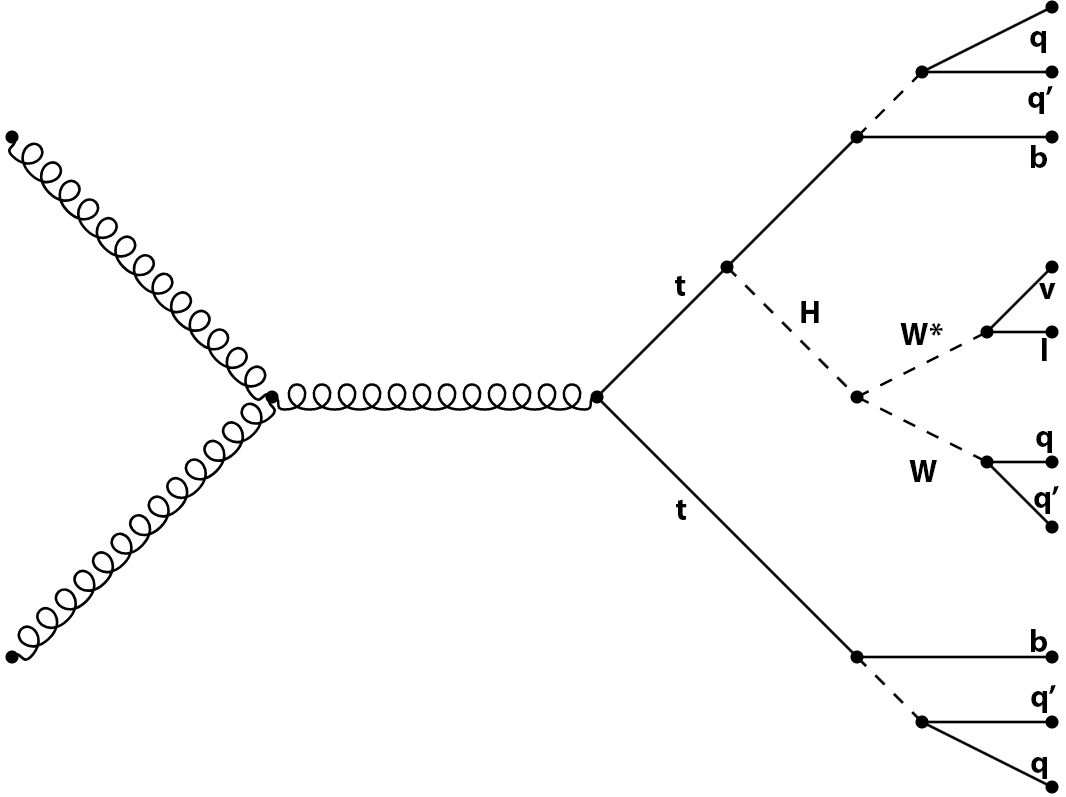
\includegraphics[width=.61\textwidth]{figures/feynman/ttH_labeled.png}
    \caption{Feynman diagram of the targeted \ttHWW event topology.}
    \label{fig:feynman_tthww}
\end{figure}


% This channel offers insight into the spin coupling between the spin-0 \Hboson and its to decay spin-1 $W$ bosons as discussed in Sec.~\ref{sec:theory:bosons}. Furthermore, additional measurements on the top Yukawa $tH$ coupling \cite{theory:why_tH_coupling} or Higgs decay branching ratios are possible using this channel. However, due to the targeted Higgs decay mode, the missing energy due to the $\nu$ in the final state as well as the off-shell $W^*$ boson pose a challenge for the event reconstruction. 


\chapter{Experimental Setup}
\label{ch:experimental_setup}
To collect data on \ttHWW events, a high-energy particle collider is necessary. Additionally, a setup for signal detection and suitable reconstruction algorithms are required. This chapter introduces the Large Hadron Collider in Sec.~\ref{sec:exp:lhc} which is used for collecting the data for this project. It is one of the most important particle accelerators worldwide and includes many experiments such as the \atlas experiment. The \atlas experiment provides the data for the project and is discussed in great detail in Sec.~\ref{sec:exp:atlas}. Other experiments are briefly described in Sec.~\ref{sec:exp:other_experiments}.

\section{Large Hadron Collider}
\label{sec:exp:lhc}
The Large Hadron Collider (\lhc) \cite{lhc_01,lhc_02} is the world's largest and most powerful particle accelerator. It's located underground near Geneva, Switzerland, straddling the border between Switzerland and France. Specifically, it's situated at the European Organization for Nuclear Research (\cern). The collider spans 27\,km in circumference and reaches depths of up to 175\,m. Along the collider, there are several detectors build which will be explored in Sec.~\ref{sec:exp:atlas} and Sec.~\ref{sec:exp:other_experiments}. Figure~\ref{fig:lhc_aerial_view} shows and aerial view of the regions above the \lhc demonstrating its size and showing the position of the different experiments.

It is used to create and accelerate bunches of protons close to the speed of light. Then a collision of these bunches is induced. During such a collision, partons from the protons interact and give rise to a large multitude of processes. By studying the debris produced by these collisions, physicists can gain insights into fundamental questions about the nature of the universe. Moreover, predictions of the SM introduced in Ch.~\ref{ch:standard_model} can be tested with such collisions. 

\begin{figure}[t]
    \centering
    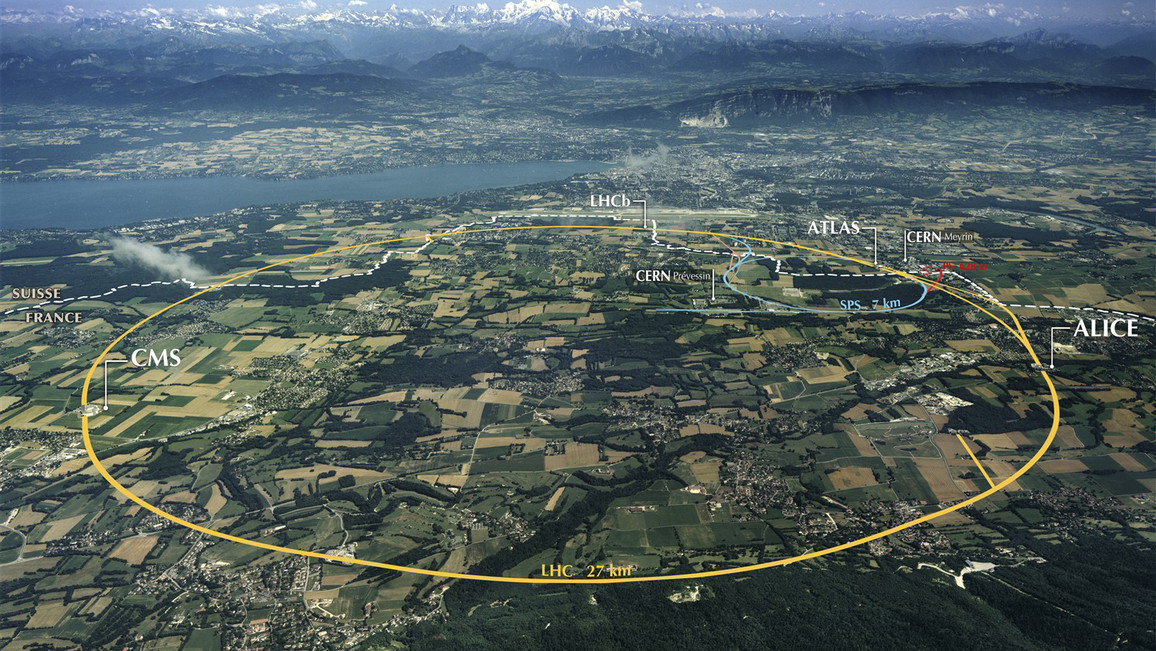
\includegraphics[width=.80\textwidth]{figures/lhc/lhc_overview.jpg}
    \caption{Aerial view above the Large Hadron Collider showing its size. The different experiments are marked along the \lhc course. \copyright{\cern}}
    \label{fig:lhc_aerial_view}
\end{figure}

The \lhc is operating for certain time periods with long shutdowns in between. The first operation period, Run~I \cite{lhc_run1}, which was active from November 2009 until February 2013. It started with a beam energy of 1.2\,TeV which was then later increased to 3.5\,TeV. In the last year it reached a beam energy of 4\,TeV. During the operation, 5.6\,fb$^{-1}$ had been accumulated by \atlas and \cms. Additionally, 1.2\,fb$1{-1}$ had been accumulated by \lhcb. Then Long Shutdown 1 followed Run~I. 

In April 2015, Run~II \cite{lhc_run2} started. The second run reached beam energies of 6.5\,TeV and lasted until December 2018. It acquired an integrated production of 160\,fb$^{-1}$. The Long Shutdown 2 then held on until 2022. 

The currently active Run~III \cite{lhc_run3} launched in April 2022 with a centre-of-mass energy of 13.6 TeV, 6.8 TeV per beam. It is planned to operate until the coming Long Shutdown 3 planned for 2026. 


\section{The ATLAS Experiment}
\label{sec:exp:atlas}
\atlas (A Toroidial \lhc ApparatuS) \cite{atlas} is one of the four main experiments at the \lhc. Its detector is designed as a general-purpose detector to explore a wide range of physics phenomena \cite{atlas:tech_design_report_01,atlas:tech_design_report_02}. The detector began its operation along the start-up of the \lhc. It spans a height of 25\,m and a length of 44\,m. It is build almost hermetically around the \lhc beam pipe as a toroidal shape which can be seen in Fig.~\ref{fig:atlas_overview}. Constructing the detector so close to the interaction point allows measuring the maximum possible phase space. Within the detector, there are several layers that are explained in great detail in Sec.~\ref{sec:exp:atlas_detector}. The coordinate system used in \atlas is important for this project and is explained in Sec.~\ref{sec:exp:atlas_coordinate_system}.


\begin{figure}[t]
    \centering
    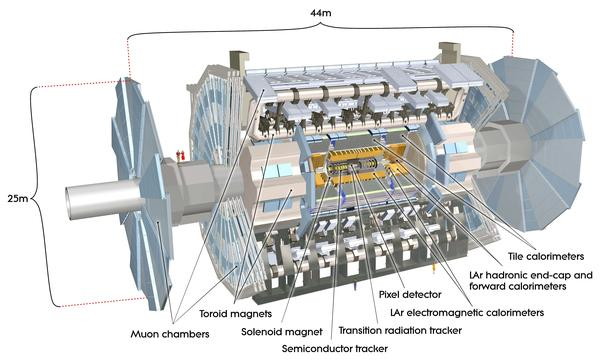
\includegraphics[width=.61\textwidth]{figures/lhc/atlas_overview.jpg}
    \caption{Overview of the \atlas detector showing its size and structure. Moreover, every important component is labelled. \copyright{BMBF}}
    \label{fig:atlas_overview}
\end{figure}

\subsection{Detector}
\label{sec:exp:atlas_detector}
The detector of the \atlas experiment is of particular interest. The following sections will cover its elements including the detector modules and magnetic systems in great detail. An overview of the detector is shown in Fig.~\ref{fig:atlas_overview}. The individual layers of the detector are further visualised in Fig.~\ref{fig:atlas_layers}. 

\begin{figure}[t]
    \centering
    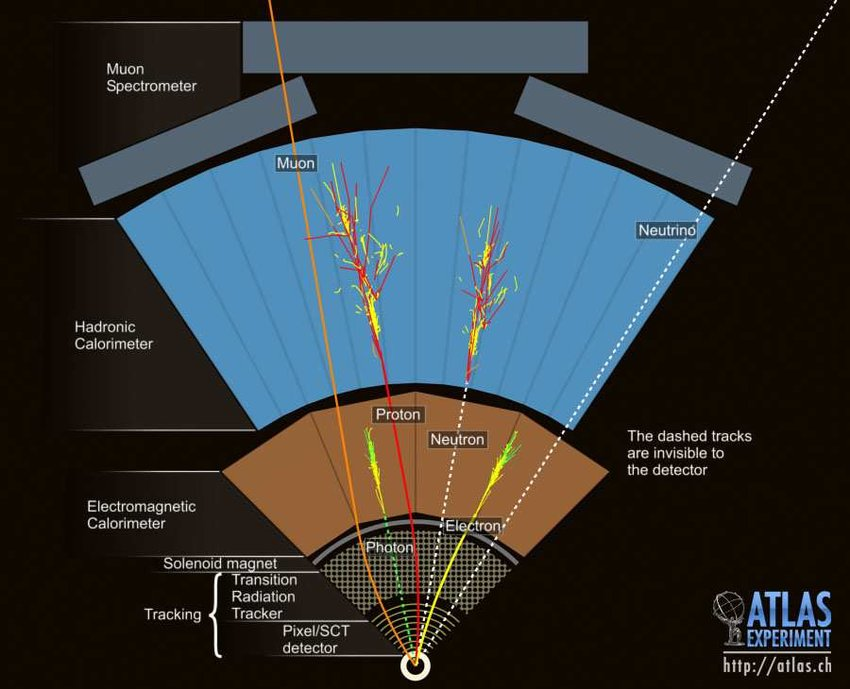
\includegraphics[width=.61\textwidth]{figures/lhc/atlas_layers.png}
    \caption{Cross-section of the concentric layers within the \atlas detector. \copyright{\cern}}
    \label{fig:atlas_layers}
\end{figure}

\subsubsection*{Magnetic System}
For the measurement of particle trajectories and their curvature, significant magnetic fields are required. For that reason, \atlas implemented superconducting magnet system build from Aluminium, Copper and Niobium-Titanium. alloy. 

It includes a central solenoid magnet surrounding the Inner Detector. It provides a central field of 2\,T \cite{atlas:tech_design_report_01}. Since the central solenoid is placed right before the calorimeter, this magnet is build as thin as possible. 

Furthermore, three large air-core toroids generate an additional magnetic field for the outer muon spectrometer. Each consisting of eight symmetrical coils placed radially around the beam axis \cite{atlas:tech_design_report_01}. These magnet systems are cooled using liquid Helium at 4.5\,K \cite{atlas:tech_design_report_01}. 

\subsubsection*{The Inner Detector}
The Inner Detector \cite{atlas:tech_design_report_inner_01,atlas:tech_design_report_inner_02} is a combined system of high-resolution detectors close to the beam pipe and continuos tracking elements at outer radii. Its task is to measure the particles' momentum. As mention before, the complete Inner Detector is surrounded by the 2\,T central solenoid magnet. Charged particles are deflected inside the detector, due to the Lorentz force. By precisely measuring the curvature, momentum measurements and particle track reconstruction are achieved.

All modules are placed either in the barrel or the end-cap region. The first region is arranged on concentric cylinders surrounding the beam axis and typically covers the low $\eta$ region. The later region's detectors are installed on disks perpendicular to the beam axis and cover the remaining space for a full coverage up to $\eta\pm2.5$.

The innermost detector tiles are semiconductor pixel detectors \cite{atlas:tech_design_report_01,atlas:pixel_detector}. The first barrel layer is only 4\,cm from the beam pipe, covers an area of 0.2\,m$^2$ and measures the complete space up to $\eta=\pm2.5$. It reaches a resolution of $\sigma_{R\phi}=12\,\mu\text{m}$ and $\sigma_{z}=66\,\mu\text{m}$. This layer is followed by two more barrel layers that cover $\eta=\pm1.7$ and reach the same resolution. To compensate this lower $\eta$ acceptance, 5 end-cap disks are placed in each side. These cover the remaining space up to $\eta=\pm2.5$. Each module is only 21.4\,mm wide and 62.4\,mm long containing 61440 pixels controlled 16 chips. Every pixel detector has its individual circuit including buffering to store data until the trigger decision. While the precision and radiation resistance of these pixel detectors are remarkable, they also introduce some material before the calorimeters and are expensive. Hence, the amount of pixel detectors that can be included in the detector is limited. 

Directly surrounding the pixel modules, the silicon strips are introduced \cite{atlas:tech_design_report_01,atlas:strip_detector}. It is subdivided into four barrel layers for the $\eta$ range up to $\eta=\pm1.4$ and 9 end-cap wheels on each side for the remaining space up to $\eta=\pm2.5$. They achieve slightly lower precision compared to the pixel modules with resolution achieving $\sigma_{R\phi}=16\,\mu\text{m}$ and $\sigma_{z/R}=580\,\mu\text{m}$. Each detector is 6.28x6.40\,cm$^2$ in size and includes 768 strips. Moreover, each module consists of four of these silicon detectors.

Straw tube trackers around the previous modules allow for a lot of measured tracking points \cite{atlas:tech_design_report_01,atlas:transition_detector}. In the barrel regions, these are placed parallel to the beam axis. In contrast to the end-caps where these are aligned perpendicular to the beam axis. Previously, these were filled with a Xenon gas mixture. However, due some leakage this Xenon was changed to Argon to reduce costs. While these achieve significantly worse resolutions of $\sigma=170\,\mu\text{m}$, they can cover a greater area to their lower cost and less material per tracking point. Hence, they strongly contribute the precise momentum measurements.

\subsubsection*{The Calorimeters}
The calorimeters \cite{atlas:tech_design_report_01,atlas:calorimeter} are used to detect charged particles by absorbing them, allowing for a measurement of their deposited energy. The physical process of showering which allow such measurements was previously described in Ch.~\ref{ch:standard_model}. \atlas' calorimeter system is subdivided into four parts: electromagnetic calorimeter, hadronic barrel calorimeter, hadronic end-cap calorimeter and hadronic forward calorimeter.

The first of these calorimeters, the electromagnetic calorimeter \cite{atlas:tech_design_report_01}, is built from Lead, liquid Argon and Kapton electrodes. It covers the pseudorapidity range up to $\eta=\pm3.2$ while the barrel region can detect up to $\eta=\pm1.475$. It is the innermost calorimeter and is primarily responsible for detecting photons and electrons. 

The hadronic calorimeter \cite{atlas:tech_design_report_01} is build around the electromagnetic calorimeter and is build from plastic scintillator plates and Iron absorber in the barrel region and from Copper, Lead and liquid Argon in the end-cap regions. This separation is done to optimise the detector for the varying requirements of the great $\eta$ range. The barrel region reaches up to $\eta=pm1.7$ and the end-caps up to $\eta=\pm3.2$. Its thickness is one of the most important parameters for the calorimeter, since it has to be suffieciently thick to contain the hadronic showers and thus, minimize punch-trough into the adjacent Muon Spectrometer.

The forward hadronic calorimeter \cite{atlas:tech_design_report_01} is implemented to cover the strongly boosted region of $3.1<|\eta|=4.9$. It as well is build from a Lead liquid Argon mixture with additional electrodes from Copper or a Tungsten alloy.

\subsubsection*{The Muon Spectrometer}
The outermost measurement part of the \atlas detector is the Muon Spectrometer \cite{atlas:tech_design_report_01,atlas:muon_chamber}. It bends the muon tracks by utilising the previously explained air-core magnets. The magnetic field is mostly orthogonal to the muon trajectories. In the region up to $\eta=\pm1.0$ the large barrel toroid magnet provides the needed magnetic field. Within the acceptance range of $1.4\leq|\eta|\leq2.7$ two smaller end-cap magnets bend the tracks. Between of these regions is the transition region where the deflection of the muon trajectories is done by the magnet field of both magnetic systems. The muon spectrometer consists of four parts.

The first part is the monitored drift tube chamber which make up 800\,m$^3$ in volume. It consists of 30\,mm diameter aluminium tubes operating with a mixture of 93\% Argon and 7\% CO$_2$. The single-wire resolution is $\sim$80\,$\mu$m. To increase the overall resolution, multilayer pairs of multiple tubes are utilised.

The New Small Wheel project replaced the original Cathode Strip Chambers \cite{atlas:muon_chamber,atlas:muon_chamber_upgrade,atlas:new_small_wheel}. It was installed after Run~II and uses Micro-Mesh Gaseous Structure as well as small-strip thing gab chambers. The former being a detector consisting of a planar electrode and a thin steel mesh forming a drift chamber. It is filled with the same Argon-CO$_2$ mixture as the first drift tube chamber. Its spatial resolution reaches 73\,$\mu$m. The later thing gab chambers consist of a Gold-plated Tungsten wire grid placed between two electrodes. The electrodes are made from a Carbon-epoxy mixture. The detector module reaches a spatial resolution of 100\,$\mu$m at the rate of up to 20\,kHz/cm$^2$.

The resistive plate chambers \cite{atlas:tech_design_report_01,atlas:muon_chamber,atlas:muon_chamber_upgrade} are another gaseous detector. It uses a non-flammable C$_2$H$_2$F$_4$ SF$_6$ gas mixture. Again, the electrodes of the detection chamber are made from Carbon. The panels themselves are made polystyrene placed between Aluminium sheets. They achieve a spatial resolution of 1\,cm and a temporal resolution of 1\,ns.

The thin gab chambers \cite{atlas:tech_design_report_01,atlas:muon_chamber} are the last chamber of the muon spectrometer. It is a proportional chamber using a flammable gas mixture of 55\% CO$_2$ and 45\% n-pentane. Even though it needs additional safety precautions, it is less sensitive to mechanical deformations, yields nearly Gaussian pulse height distributions and has a small dependence on the incident angle. The distance of both electrodes are 2.8\,mm.

\subsubsection*{Trigger System}
The aforementioned detector systems are able to detect and record significant amounts of data. The initial interaction rate of $\sim$1\,GHz resulting in a bunch-crossing rate of up to 40\,MHz \cite{atlas:tech_design_report_01} are too much to save. Approximately only 0.1\,kHz of data is suited for permanent storage. Thus, a very fast selection must be defined and implemented that discards most of the events to a manageable level. For that purpose, an online multi-level trigger system is introduced. Each trigger level refines the selection done from the previous level.

The first level (LVL1) trigger \cite{atlas:tech_design_report_01,atlas:trigger_lvl_1} makes the initial selection. It utilises several subsets of detectors with reduced resolution to quickly decide whether the recorded event is saved or discarded. This is done by identifying potential candidates. The LVL1 decision is then based on certain object requirements. The maximum rate for the LVL1 trigger is up to 75\,kHz, targeting a decision latency of up to 2\,$\mu$s. The selected events of the LVL1 trigger are temporary saved into readout drivers and then readout buffers. 

The event data stays on the readout buffers until the LVL2 trigger \cite{atlas:tech_design_report_01,atlas:trigger_lvl_high} either rejects or accepts them. The second trigger level utilises the region-of-interest information provided by the LVL1 trigger. It includes information on the position and momentum of potential objects and the sums of transverse energies $E_T$ and $E_T^\text{miss}$. The LVL2 trigger uses only the necessary information but has access to the full resolution information from the detectors. The LVL2 trigger reduces the rate to around 1\,kHz. Its latency is variable but in the range of 1-10\,ms. Events that pass both triggers are then transferred to an offline event filter system that performs the final selection. The final output data rate is approximately 100\,MB/s.


\subsection{Coordinate System}
\label{sec:exp:atlas_coordinate_system}
The \atlas detector is built as a cylinder. Thus, a fitting coordinate system must be defined. For that, every position in the detector is defined by the $z$ position parallel to the beam axis, the azimuth angle $\phi$ along the detector and the pseudo-rapidity $\eta$ with respect to the collision point of the detector. Figure~\ref{fig:atlas_coordinate_system} shows qualitatively how the detector coordinate looks like when the detector cylinder is rolled out and projected onto a 2 dimensional plane. 

\begin{figure}[t]
    \centering
    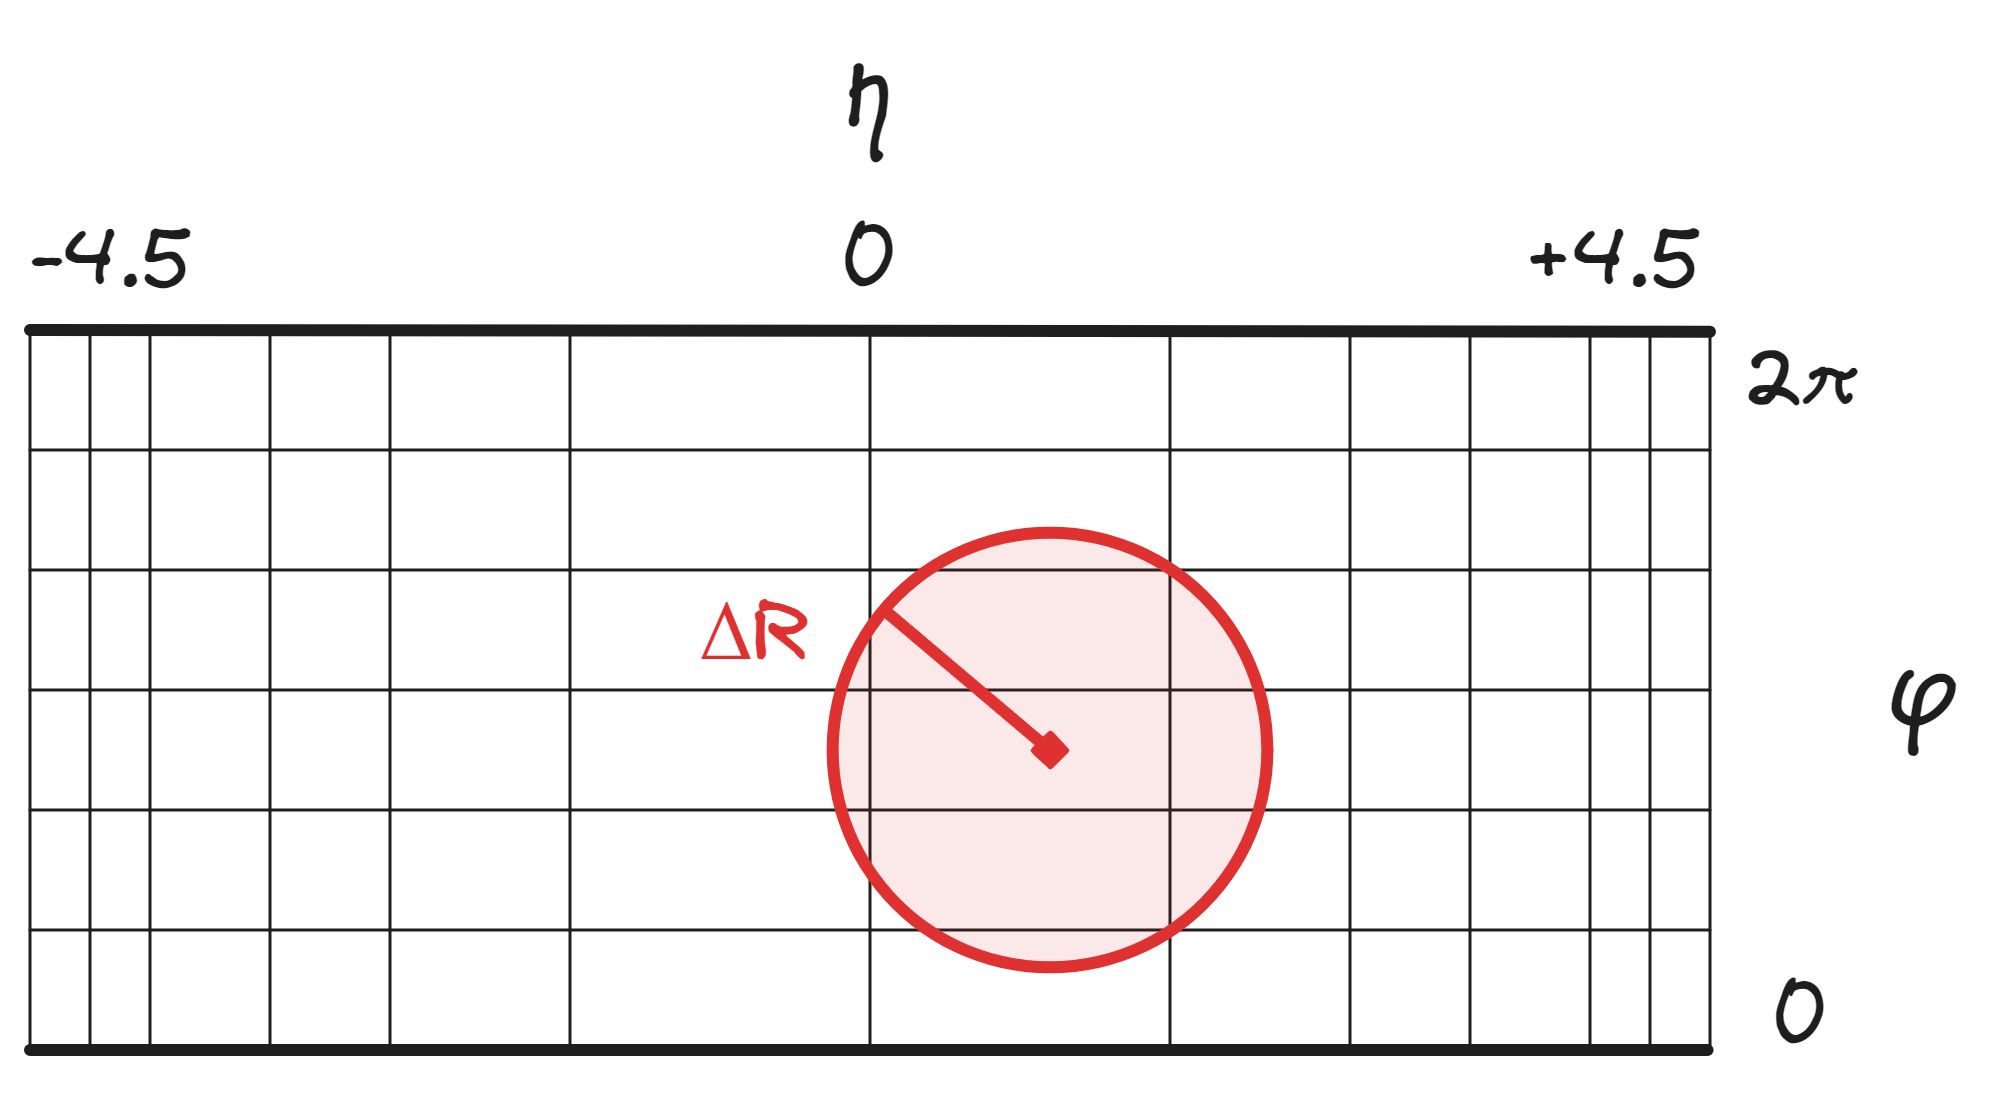
\includegraphics[width=.80\textwidth]{figures/lhc/atlas_coordinate_system.excalidraw.png}
    \caption{Sketch visualising the \atlas coordinate system using the azimuth angle $\phi$ and pseudo-rapidity $\eta$. It represents the rolled out detector cylinder. Moreover, it shows how a spatial cone defined by $\Delta R$ would look like.}
    \label{fig:atlas_coordinate_system}
\end{figure}

To properly work with spatial separations in this coordinate system, the variable

\begin{align}
    \Delta R &= \sqrt{\left(\Delta \phi\right)^2 + \left(\Delta \eta\right)^2}\label{eq:delta_r}
\end{align} 

is introduced. It represents a cone around each point in the coordinate system as shown in Fig.~\ref{fig:atlas_coordinate_system}. This should not be confused with $R$ which is typically the radius from the beam pipe. Hence, expressions such as $R\phi$ correspond to the radial scaled azimuth angle and is used in classifying detector resolutions as seen before.

\section{Other Experiments}
\label{sec:exp:other_experiments}
Besides the discussed \atlas experiment, there are three more main experiments at the \lhc: \cms, \alice and \lhcb. This section will briefly mention each of these experiments and compare them to the \atlas experiment.

The \cms (Compact Muon Solenoid) \cite{other:cms} detector is a general-purpose similar to the \atlas detector. Its detector is shown in Fig.~\ref{fig:detector_cms}. As its name suggest, a particular focus is set on the precise measurement of high energy muons over a wide range of angles and momenta. Its main goals include muon mass resolution of around 1\% at 100\,GeV and the ability to determine the charge of muons with momentum $p$<1\,TeV. Other main goals include the reconstruction of charged particles, efficient tagging of $\tau$ leptons and $b$ quarks, precise missing transverse energies and isolation of photons and leptons at high luminosities. \cms started its operation with the commissioning of the \lhc.

\begin{figure}[t]
    \centering
    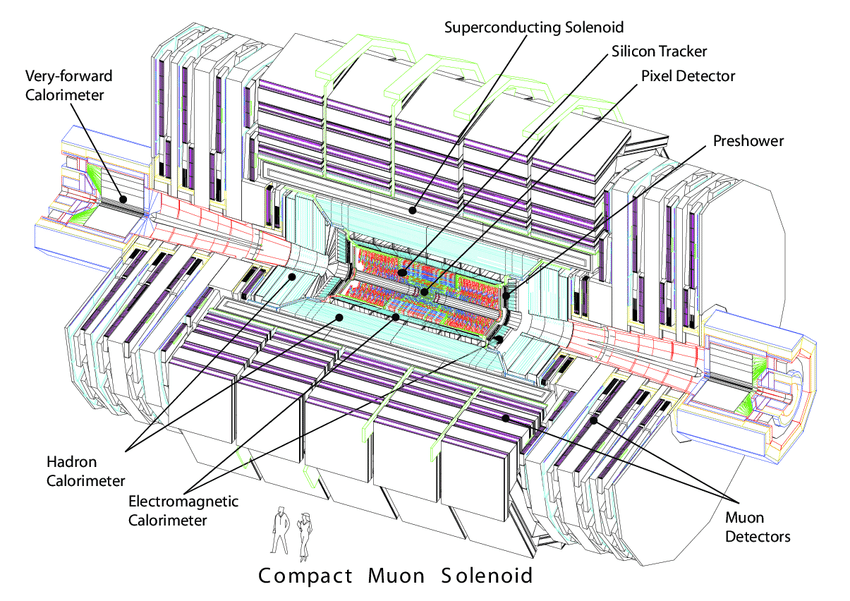
\includegraphics[width=.8\textwidth]{figures/lhc/detector_cms.png}
    \caption{Overview of the \cms detector \copyright{\cern}}
    \label{fig:detector_cms}
\end{figure}

The \alice (A Large Ion Collider Experiment) \cite{other:alice} focuses on heavy ion collisions. It is designed to measure the physics of strongly interacting matter and the quark-gluon plasma at extreme energies and temperatures. It consists of a central barrel which covers polar angles from 45$^\circ$ to 135$^\circ$ and a forward muon spectrometer covering 2$^\circ$ to 9$^\circ$. The detector layout is further visualised in Fig.~\ref{fig:detector_alice}. While the \alice physics program includes the study of light atoms, the main study utilises heavy nuclei Lead-Lead collisions. Its first collisions was recorded in November 2010.

\begin{figure}[t]
    \centering
    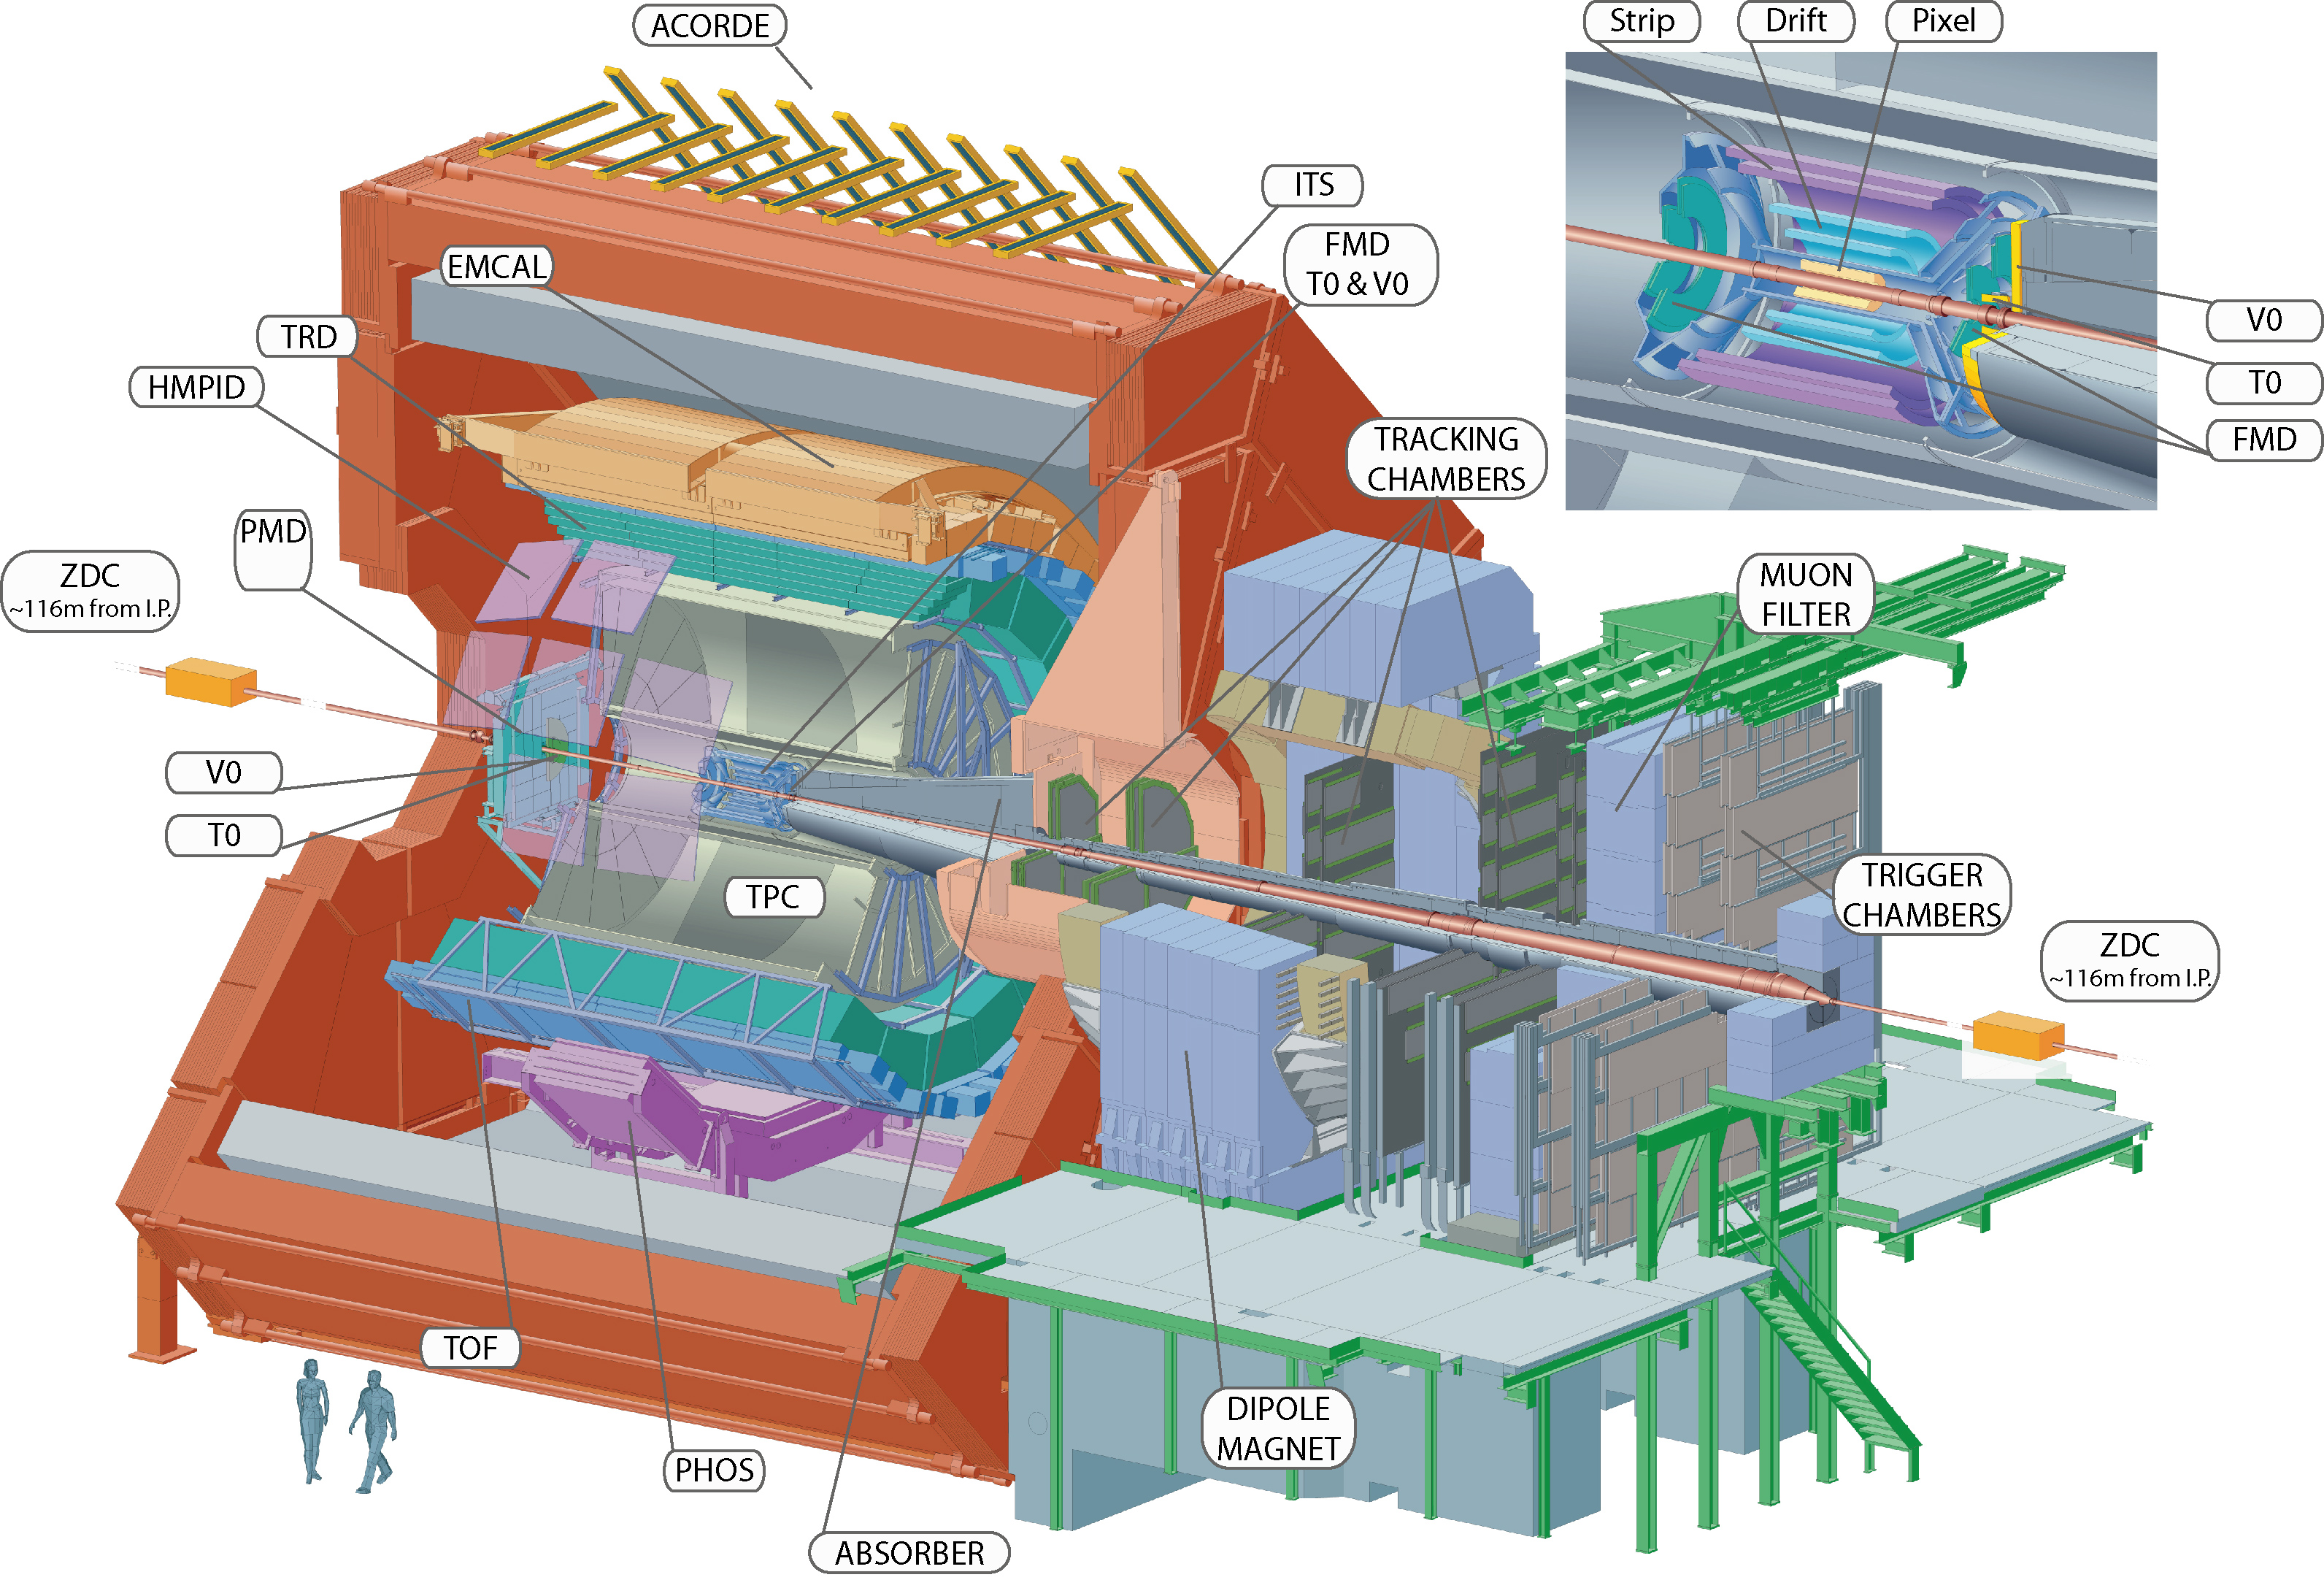
\includegraphics[width=.8\textwidth]{figures/lhc/detector_alice.jpg}
    \caption{Overview of the \alice detector \copyright{\cern}}
    \label{fig:detector_alice}
\end{figure}

\lhcb (Large Hadron Collider beauty) \cite{other:lhcb} is dedicated to study particles that contain $b$ quarks, which sometimes are referred as beauty quarks. Unlike the other experiments, its detector is build as a single-arm spectrometer which can be seen in Fig.~\ref{fig:detector_lhcb}. It covers a forward angle of approximately 0.5$^\circ$ to 17$^\circ$. The reason lies in \lhcb's focus on detecting $b$ hadrons which are predominantly produced in forward and backward cones. The \lhcb experiment started the operation at the same time as \atlas and \cms.

\begin{figure}[t]
    \centering
    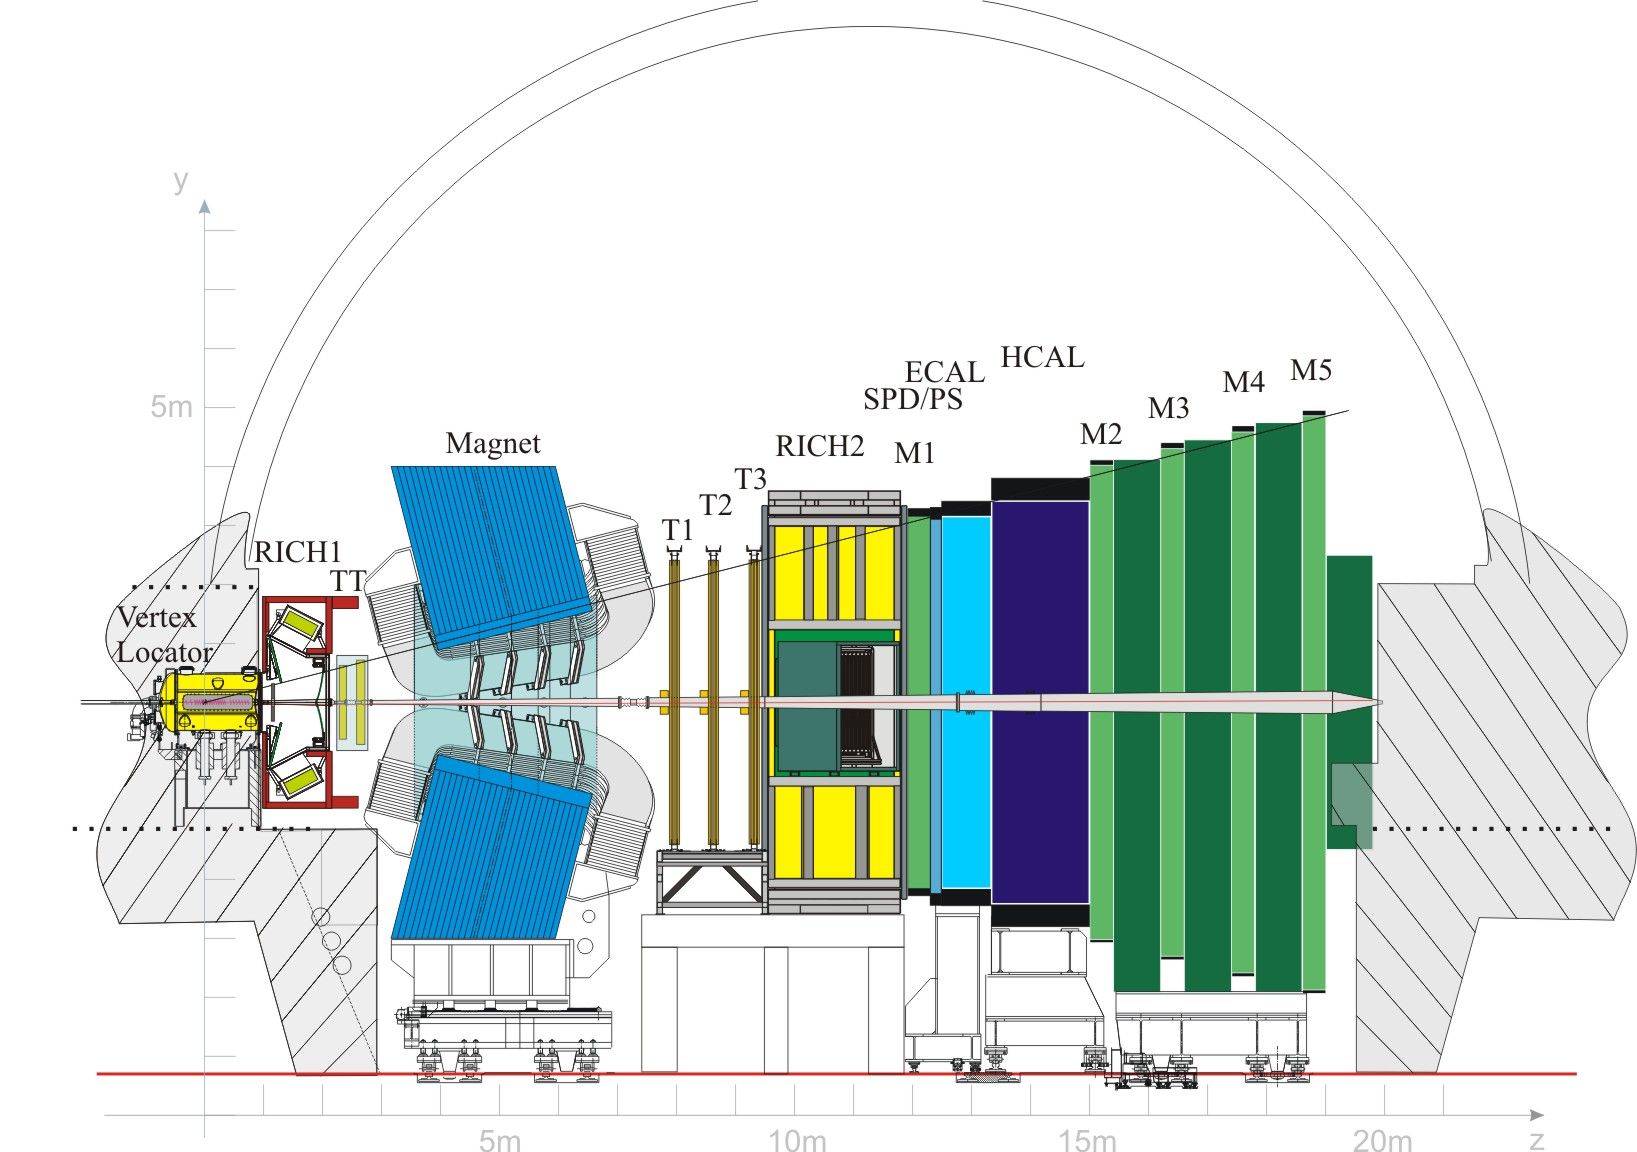
\includegraphics[width=.8\textwidth]{figures/lhc/detector_lhcb.jpg}
    \caption{Overview of the \lhcb detector \copyright{\cern}}
    \label{fig:detector_lhcb}
\end{figure}


\chapter{Deep Neural Networks}
\label{ch:neural_networks}
Deep neural networks (DNN) are a modern technique for many different analysis. Unlike classical algorithms, neural networks are designed to adapt to a given dataset. This adaptation simulates a learning process and hence provides the possibility to train neural networks for certain tasks. Machine learning approaches are widely used in several fields of studies and can be used in particle physics as well. 

Modern neural networks are algorithms which simulate multi-layered DNNs inspired by the original Perceptron \cite{nn:perceptron} with several hidden layers between the input and output layer. Figure~\ref{fig:neural_networks} shows so-called feedforward neural network which is a simple neural network design. In a feedforward DNN each node of a layer receives a weighted input from every node of the previous layer and emits an output, which will be used in the next layer \cite{nn:node_calculation}. The output of the hidden layers are usually not stored and thus invisible.

This idea can be described mathematically using a vector $\vec{v}$ for input and $\vec{u}$ for output. The length of these vectors correspond to the number of nodes in the first and last layer \cite{nn:node_calculation}. Each node has $n$ inputs $x_i$, corresponding weights $w_i$ and an offset $b$ which are all used to calculate the raw activation

\begin{align}
	z = \sum_i^n w_ix_i + b\,.
\end{align}

The raw activation $z$ is used in a chosen activation function $f$ to produce an output $a$ \cite{nn:node_calculation}. %This process per node is shown in Figure~\ref{fig:neural_networks}. Common choices for the activation function $f(z)$ are \textit{tanh}, \textit{Sigmoid}, \textit{ReLU} and \textit{Softmax} \cite{nn:activation_function}. 

To train a DNN, the given dataset is usually divided into a training and a validation set. The first set is used in the training process to teach the neural network. Each step, a certain batch of samples are used for training the DNN. After the whole training set is used, an epoch is completed and the performance of the neural network is tested on the statistically independent validation set. The improvement for a given epoch is determined by the loss which needs to be minimised \cite{nn:overfitting}. If the neural network trains for too many epochs on a given training dataset, it begins to overfit. This means, the DNN improves its performance on the training set, but worsens on validations sets \cite{nn:overfitting}. Overfitting can be prevented by including some regularisation technique such as early stopping. 

\begin{figure}[t]
	\centering
	\includegraphics[width=.52\textwidth]{figures/methods/nn_map.png}\hfill
	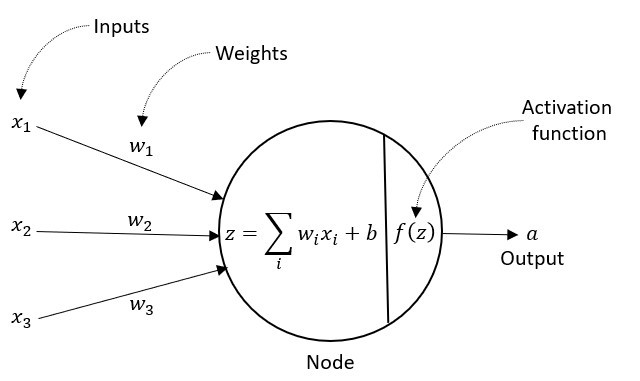
\includegraphics[width=.47\textwidth]{figures/methods/nn_node.png}
	\caption{A schematic visualisation of a DNN (left) using one hidden layer. Each node can be represented (right) with multiple weighted inputs and an activation function $f$.}
	\label{fig:neural_networks}
\end{figure}


\section{SPA-Net}
\label{sec:neural_networks:spanet}
Traditionally, to determine a jet-parton assignment, the classical $\chi^2$ minimisation approach \cite{nn:chi_squared} is used. For top analysis in particular, this was calculation was implemented in the KL-Fitter framework \cite{nn:kl_fitter}. For this project, the method would be deployed by testing every possible combination of jets, calculating the masses $M$ of the resonance particles ($t$,$W$,$H$) and then compare it to the SM prediction $m$. Mathematically, for every assignment one must calculate

\begin{align*}
    \chi^2 = \sum_{i,j} \frac{(M_{q_i}-m_j)^2}{\sigma_j^2}
\end{align*}

with $\sigma$ being the SM mass uncertainty. The lowest $\chi^2$ value corresponds to the best jet-parton assignment. However, this approach is not suited for a channel with manly jets in the final state due to the high number of permutations. Instead, a neural network is implemented.

For this project, the transformer DNN \spanet (Symmetry Preserving Attention Networks) \cite{spanet_01,spanet_02} is used to predict the hadronic jet-parton assignment. \spanet was originally used in a fully hadronic \ttbar analysis \cite{spanet_03}. The implemented is optimised for general event topologies \cite{spanet_01} and thus, can be used for the targeted \ttHWW topology.  

Its task is to predict a jet-parton assignment for all jets in the final jets. This assignment can then be combined with the leptonic prediction by neutrino weighting as explained in Ch.~\ref{ch:neutrino_weighting} resulting in a full event reconstruction.

\spanet utilises symmetries in the event topology. Symmetries are classified into two groups: jet and particle symmetries. The jet symmetry describes that labelling of certain particles is symmetric and thus, changing their labels does not change their physical behaviour. In the \ttHWW topology, this symmetry is present in the $W$ boson decays which produce two quarks $q\bar{q}'$. Under the assumption, that the $W$ couples evenly to both quarks, their labelling can be changed without any physical consequence. The particle symmetry depict the symmetry in respect to the particle origin. This means, particles that originate from a quark or its respective antiquark are symmetric, when disregarding their charge. Since the charge of a jet is difficult to measure, this symmetry is functional. 

By considering these symmetries, the number of possible permutations is reduced and the processing speed increases. These symmetries are implemented in the symmetric cross entropy loss during training. Changes which obey these symmetries do not change the loss value.

\spanets architecture of this neural network is visualised in Fig.~\ref{fig:spanet}. It can be subdivided in to four components \cite{spanet_01}: jet input embeddings, central transformer, particle transformers and self-attention output layer.

\begin{figure}[t]
    \centering
    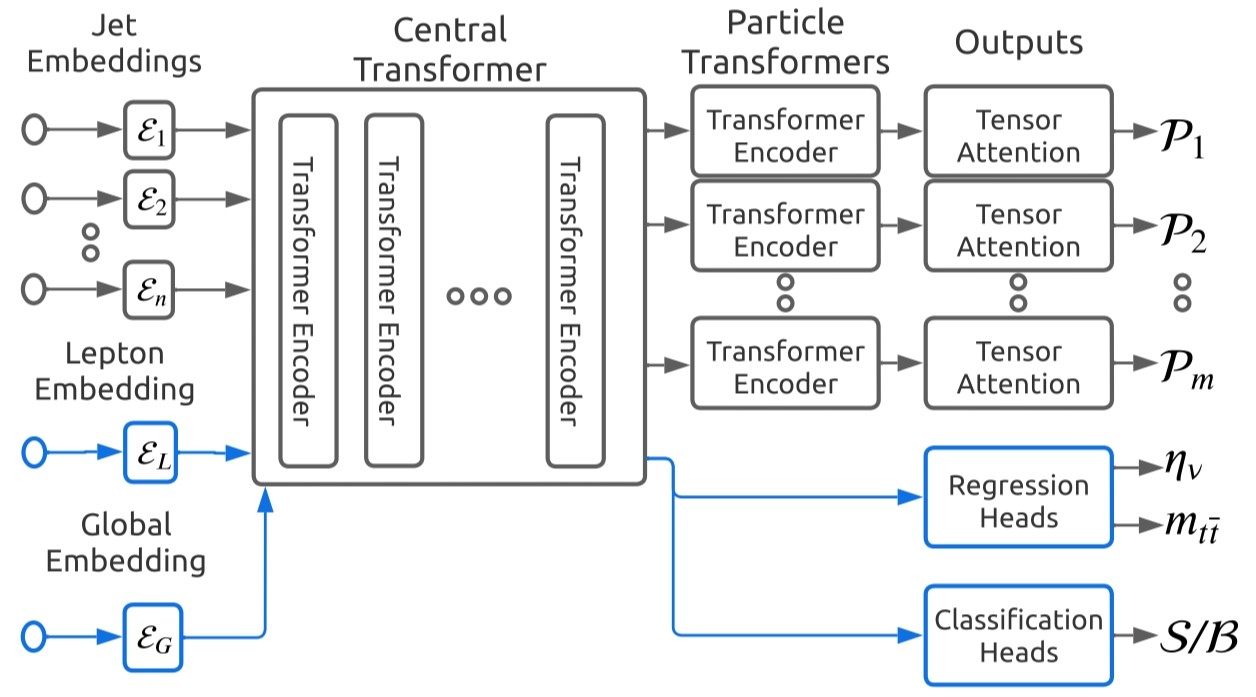
\includegraphics[width=.85\textwidth]{figures/methods/spanet_architecture_2.jpg}
    \caption{Overview of \spanets architecture including its four regions and the additional embeddings for lepton and global information \cite{spanet_02}.}
    \label{fig:spanet}
\end{figure}

During training, each prediction is split into three steps. First, the amount of valid jet assignment permutations is reduced by splitting up event into sub-structures which are predefined by the event topology. Then each jet-parton assignment sub-problem is solved by applying a `Symmetric Tensor Attention' \cite{spanet_01} layer. It produces a single tensor all possible assignments containing the probabilities that any particular combination is the correct sub-assignment. These tensors are combined into a final jet-to-patron prediction by calculating the combined symmetric loss \cite{spanet_01}. The approach of splitting up the individual particles allows partial event reconstruction. These partial events can be used in training since they still provide impactful training signal.

During inference, the combined symmetric loss is not calcluated. Instead, \spanet iteratively assigns jets to the to expected particles. For each assignment, its corresponding score is calculated. During these permutations, no jet can be assigend to multiple particles to ensure a unique jet-parton assignment.

In comparison to other assignment techniques, \spanet offers several advantages: \cite{spanet_01}

\begin{itemize}
    \item The network is agnostic to the number of input objects (jet multiplicity). Hence, training and prediction can be done with samples that contain events with different number of jets.
    \item All predicted jet matches are unique. No object is matched to more than one jet. Furthermore, each prediction is also rated using an assignment probability that represents \spanets confidence for that particular prediction.
    \item Expected symmetries due to the event topology can be predefined. These symmetries are then preserved and used to speed up the process by simplifying the prediction task. 
\end{itemize}

To train and fine-tune \spanet to the targeted topology, a fitting training sample must be created. This necessitates the development of a truth matching algorithm which is introduced in Ch.~\ref{ch:truth_matching}.


\chapter{Neutrino Weighting}
\label{ch:neutrino_weighting}
Neutrino Weighting is a technique to reconstruct events including neutrinos in their final state. It was first implemented by the \dzero collaboration \cite{neutrino_weighting:original} in dileptonic \ttbar events. Events with neutrinos are typically underconstrained and need certain assumptions to be reconstructed. Neutrino weighting yields the needed constraints by calculating the most likely combination of unknown parameters. While the original neutrino weighting was developed for events with two neutrinos in the final state that need to be constrained, this project will adapt the approach to reconstruct the leptonically decaying $W^*$ boson in the \HWW subprocess \cite{neutrino_weighting:adaptation}. For the targeted event topology, the needed constraints are the off-shell mass of the $W^*$ boson and the $\eta$ of the neutrino.  

First, the mass of the Higgs boson is assumed to be fixxed at $M_H=125.09\,\text{GeV}$ \cite{pdg}. Additionally, the mass of the on-shell \wboson is assumed to be $M_W=80.379\,\text{GeV}$ \cite{pdg}. Then, to fully reconstruct the \HWW sub-structure, several combinations of the off-shell mass $M_{W^*}$ and the pseudo-rapidity of the neutrino $\eta_\nu$ will be sampled. 

Using these assumptions, the \HWW subsystem is fully constrained \cite{neutrino_weighting:adaptation} and the neutrino transverse momentum $p_T^\nu$ can be calculated. This reconstructed neutrino momentum $p^\nu$ can be compared to the observed missing momentum $p^\text{miss}$ by calculating the weight 

\begin{align}
    w = \exp{\frac{(p_x^\nu-p_x^\text{miss})^2}{\sigma_x^2}} \cdot \exp{\frac{(p_y^\nu-p_y^\text{miss})^2}{\sigma_y^2}}.
\end{align}

Here, the variable $\sigma_{x/y}$ is the experimental resolution of the missing momentum $p_{x,y}^\text{miss}$. The weight $w$ is in the range of $[0,1]$. Higher values mean better agreement between the calculated values and the observation. If the weight is calculated for many samples of $M_{W^*}$ and $\eta_\nu$, a plot as seen in Fig.~\ref{fig:neutrino_weighting} can be created. The maximum of this distribution corresponds to the most likely combination of the unknown parameters. These values will then be used for the event reconstruction.

\begin{figure}[t]
    \centering
    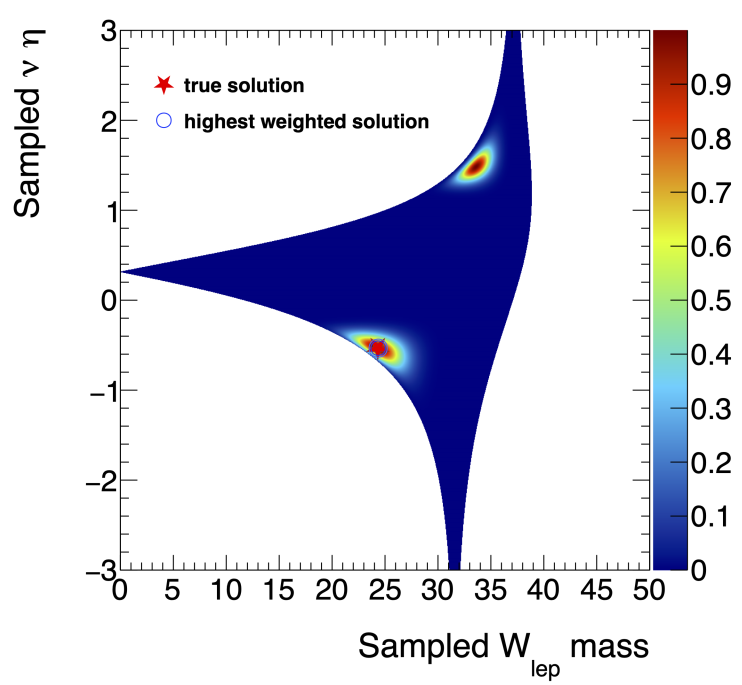
\includegraphics[width=.60\textwidth]{figures/methods/neutrino_weighting.png}
    \caption{Example plot showing a potential distribution of weights for several sampled combinations of $\eta_\nu$ and $M_{W^*}$. The most likely combination of parameters can be seen at the red peaks \cite{neutrino_weighting:adaptation}.}
    \label{fig:neutrino_weighting}
\end{figure}

Besides using the calculated weight for each event to estimate the most likely unknown parameters, it can also be used in the event selection to reduce backgrounds. Previously, this technique has been estimated to greatly suppress backgrounds in \HWW systems \cite{neutrino_weighting:adaptation} by discarding all events with a neutrino weight $w<0.7$. Using this selection, a theoretical signal purity of 20\% was calculated.


\chapter{Truth Matching}
\label{ch:truth_matching}
As mentioned in Sec.~\ref{sec:neural_networks:spanet}, training \spanet necessitates some training samples. These training samples were not available. Hence, a truth matching algorithm needs to be developed. The algorithm must take the truth and reconstructed information of well-defined MC simulations as inputs and outputs a jet-parton assignment which then can be learned by \spanet. A high-level explanation of the algorithm is given in Sec.~\ref{sec:truth_matching:algorithm}. The following Sec.~\ref{sec:truth_matching:validation} cover the validation results. 

\section{Algorithm}
\label{sec:truth_matching:algorithm}
The developed algorithm begins by scanning the input MC samples and pairing the reconstructed and truth column. The algorithm begins by iterating through all final state quarks in the truth column. For each of these partons, it searches possible jet matches. All jets within a spatial cone around a parton are considered as its candidate matches. Here, the cone is defined by $\Delta R\leq0.4$ as introduced in Sec.~\ref{sec:exp:atlas_coordinate_system}.

As for the current state of the project, only the six quarks originating from the \ttbar system are matched. This will be changed in the near future to also include the two quarks from the hadronic part of the \HWW decay.

If there is no jet within the cone of one parton, then the corresponding particle is not be matched. If exactly one candidate is found inside the cone, the jet is saved as the final match for the jet-parton assignment. For cases with more than one candidate match, an additional step has to be implemented to decide which of the candidates is selected.

To select a partons final match from multiple candidates, a metric must be defined. Then, the algorithm will choose the jet from those candidates, which optimises the chosen metric. In this step, different metrics were tested and compared as explained in Sec.~\ref{sec:truth_matching:validation}. 

Each matched jet is made unavailable for other partons. Hence, each jet-parton assignment is unique which is required for training \spanet. After all partons were iterated, the algorithms proceeds to combine the matched four-vectors to the expected original resonance particles ($W$,$t$,$H$).

Currently, an event is defined as a successful match, if both top quarks - and hence all decay particles of the fully hadronic \ttbar system - are matched. Again, the \HWW subsystem is not yet included in the current truth matching version.

The algorithm utilises several technical optimisations such as bit-shifting operation. Thus, generating a matched training sample takes little time of around 30\,s for 1 million events. This is negligible compared to the time for converting a training sample in a fitting format for \spanet which takes around 2\,h for the same amount of events.

\section{Validation}
\label{sec:truth_matching:validation}
After implementing the truth matching algorithm, several validation tests were conducted which are explained in the following.

\subsubsection*{Successful Event Matches}
The first validation results can be seen in Fig.~\ref{fig:success_by_jets} which features two summarising plots that show the success rate of the matching algorithm per jet multiplicity for 1 million events. Only the success of full \ttbar matches is shown. 

More jets in the final state are expected to increase the chance for successful event matches since more jets are available. This expectation is fulfilled as seen in Fig.~\ref{fig:success_by_jets}. However, the statistics decreases for higher jet multiplicities, because every additional jet originating from some parton needs to come from some higher-order physics process with additional couplings. Events with less than 6 jets can not fully match the expected \ttbar system. Hence, these are not investigated. In the next truth matching version, this will be increased to 8 jets to include all expected final state quarks.

While many events are fully matched, all events with at least 6 jets will be used in training \spanet. This maximises the available training statistics and as mentioned in Sec.~\ref{sec:neural_networks:spanet}, \spanet can utilise partial reconstructions in its training. 

\begin{figure}
    \centering
    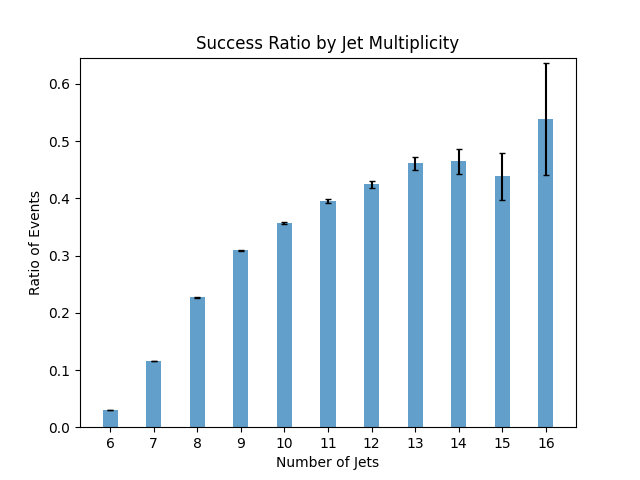
\includegraphics[width=.48\textwidth]{figures/truth_matching/success_ratio.png}\hspace{.03\textwidth}
    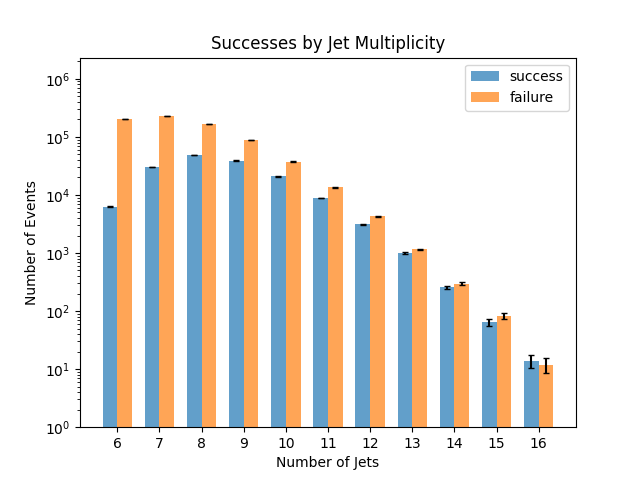
\includegraphics[width=.48\textwidth]{figures/truth_matching/success_by_jets.png}
    \caption{Overview of the total successful event count (left) and relative success rate (right) for the matching algorithm subdivided by the number of jets in the event.}
    \label{fig:success_by_jets}
\end{figure}


\subsubsection*{Final Jet Selection}
To optimise the matching in the case of multiple matching candidate per parton, three different schemes were tested. 

The first matching scheme compares the spatial separation between the potential jets and the targeted particle. The closest jet as calculated using $\Delta R$ is selected as the final match. 

The second approach focuses on the $\Delta p_T$ of the potential jets and the targeted particle. Here, the closest pair in momentum space is selected as the final match. This scheme is motivated by the CP violating properties of the \wboson which should result in non-symmetric transverse momenta for the decay particles. 

One last scheme was tested which combines the information of the $\Delta R$ and $\Delta p_T$ approach. For the combined scheme, the $\Delta R$ was scaled to a range of [0,4] and $\Delta p_t$ to a range of approximately [0,$\sim$10]. The latter one is not exact since it has no cut applied. Then, the pair that minimises the sum of both variables is chosen as the final match.

The success ratios for matching individual particles or the \ttbar system are summarised in Tab.~\ref{tab:final_selection}. It shows that the $\Delta R$ scheme performs the best. Hence, it will be used from now on. Interestingly, the different schemes change the results only by small amounts <1\,\%. Investigations showed that less than 20\,\% of events have any truth parton with more than one candidate match. Furthermore, these cases often choose the same final match regardless of the applied matching scheme. Hence, changing the matching scheme has little effect on the overall matching success rate. No further investigation into the final matching procedure was performed. 

\begin{table}
    \centering
    \caption{Overview of the three different matching schemes tested for the final jet matching. It shows the success fraction for each object and the combined \ttbar system. The highlighted $\Delta R$ only approach yields the best results.}
    \begin{tabular}{l|c|c|c|c|c|}
        &\multicolumn{5}{c|}{successful matching in \%}\\
        & $t\bar{t}$ & $t$ & $\bar{t}$ & $W_t$ & $\bar{W_t}$\\
        \hline
        \rowcolor{highlighter!40}
        $\Delta R$ only & 17.6 & 43.9 & 44.1 & 53.4 & 53.6\\
        $\Delta R$ and $\Delta p_T$ & 17.5 & 43.7 & 43.9 & 53.1 & 53.2\\
        $\Delta p_T$ only & 17.4 & 43.6 & 43.9 & 53.0 & 53.2\\
    \end{tabular}
    \label{tab:final_selection}
\end{table}

\subsubsection*{Higgs Decay Modes}
Finally, an overview of different regions defined by the event jet multiplicity and $H$/$W$ decay modes can be seen in Tab.~\ref{tab:higgs_decay}. It shows the ratio of successful matches and the relative yield for each region using a total of 4 million events.

Immediately, the difference between the $\geq5$ and $\geq6$ jets region becomes clear. While the first region with any $H$ decay and at least 5 jets in final state includes all events, the second region excludes all events with to few jets detected. Thus, it has a higher matching success rate of 17.6\,\% instead of 15.8\,\% for full \ttbar matching. To match not only the \ttbar system, but also the needed hadronic $W$ from $H$, $\geq8$ jets are needed. This region includes around 5.2\% of all events. However, the correct $H$ decay mode must still be selected.

The targeted topology is highlighted in the table and shows that around 0.11\% of all events are in this region. The low statistics could pose a problem for training \spanet. The cause for the low statistics lies in the $H$ decay identification using the event \textsc{pdgIds}. Around 90\,\% of all events including a \HWW substructure have ill-defined \texttt{pdgIds}. Hence, these events are not classified and discarded resulting in lower statistics. A new sample with fixed truth records is expected to be available later in the analysis. If the statistics for training \spanet becomes a problem in the future, this will be investigated further.

Note that the last row (fully hadronic \HWW) behaves differently than one might expect initially. The branching ratio of \wbosons would favour hadronic decays, yet no full hadronic decays are seen in the MC Simulations. While this indicates that there might be an error, investigation show that this behaviour is expected. This phenomenon originates from the implemented single-lepton trigger. Since the MC simulation includes only events where the \ttbar system decays fully hadronically and in that particular region requires the \HWW subsystem to also decay fully hadronically, there is no lepton produced. Hence, these events do not pass the trigger. This results in no event counted for that region. %This reduction is due to the fact that events with no high $p_T$ lepton are discarded and the \ttbar system is targeted to decay fully hadronically. Hence, the other high $p_T$ leptons can only originate from effects such as radiation or NLO processes. %When the \HWW subprocess does not yield any leptons, the top quarks must decay into a lepton. However, the simulations contain only fully hadronic \ttbar samples. Thus, any event with no lepton from the \Hboson is guaranteed discarded.
% This behaviour is also expected to caused by the broken \texttt{pdgIds}.

\begin{table}
    \centering
    \caption{Overview of several regions defined by jet multiplicity and decay modes showing their relative yield to the total data set and matching success rates. The last three regions are events with \HWW decays, subdivided into fully leptonic, semileptonic and fully hadronic $WW^*$ decays. The highlighted row corresponds to the targeted topology.}
    \begin{tabular}{l|r|c|c|c|c|c|}
        &&\multicolumn{5}{c|}{successful matches in \%}\\
        & rel. yield & $t\bar{t}$ & $t$ & $\bar{t}$ & $W_t$ & $\bar{W_t}$\\
        \hline
        $(\text{all})^{\text{5+ jets}}$  & 100.0\% & 15.8 & 41.0 & 41.2 & 50.5 & 50.7\\
        $(\text{all})^{\text{6+ jets}}$  & 90.1\% & 17.6 & 43.9 & 44.1 & 53.4 & 53.6\\
        $(\text{all})^{\text{8+ jets}}$  & 5.2\% & 30.1 & 56.3 & 56.5 & 62.9 & 63.1\\
        \hline
        $(H\rightarrow bb)^{\text{8+ jets}}$ & 27.4\% & 27.3 & 53.9 & 54.0 & 63.4 & 63.4\\
        $(\HWW)^{\text{8+ jets}}$ & 0.52\% & 31.2 & 56.9 & 57.4 & 63.6 & 63.8\\
        \hline
        $(\HWW)_{\text{fully leptonic}}^{\text{8+ jets}}$ & 0.41\% & 31.6 & 57.3 & 57.8 & 64.0 & 64.2\\
        \rowcolor{highlighter!40}
        $(\HWW)_{\text{semileptonic}}^{\text{8+ jets}}$ & 0.11\% & 29.6 & 55.4 & 55.8 & 62.2 & 62.3\\
        $(\HWW)_{\text{fully hadronic}}^{\text{8+ jets}}$ & 0.00\% & - & - & - & - & -\\
    \end{tabular}
    \label{tab:higgs_decay}
\end{table}


\chapter{Project Status}
\label{ch:status}
The project started on the 3rd of November 2023 and has been going for approximately 5 months so far. The progress so far is briefly summarised in \ref{sec:status:progress}. The future steps in the project as well as potential future expansions are stated in Sec.~\ref{sec:status:roadmap} and Sec.~\ref{sec:status:outlook}, respectively.  


\section{Progress}
\label{sec:status:progress}
So far, this project mainly focused on generating truth matched samples for training \spanet. The developed algorithms as well as its validation were introduced in Sec.~\ref{ch:truth_matching}.  

Furthermore, after obtaining a certificate from the `Deutsche Forschungsnetz' (DFN) and gaining access to the NAF cluster, \spanet was installed alongside some training samples of different sizes. Some complications due to disk space and incompatible driver versions slowed down the implementation. 

The workflow for generating samples to train and fine-tune \spanet has now been established. The first training ran successful job. Only some minor modifications are still needed to include the hadronic part of the \HWW subsystem into the training workflow. 


\section{Roadmap}
\label{sec:status:roadmap}
Since the initial workflow has now been established, the next project steps will be initiated. After including the assignment of the hadronic \HWW decay into the truth matching, the training samples for \spanet will be regenerated. Using these new samples, several versions of \spanet will be trained independently. These versions differ by their choice of hyperparameters and will be compared to find the best performing network. The optimised version of \spanet will be used as the final model. After the hyperparameter optimisation, \spanet will be trained on a greater dataset. While these \spanet versions train on the NAF cluster, the neutrino weighting will be implemented and validated. As soon as these two steps are done, they can be merged for a full event reconstruction. These goals are summed up in the following roadmap.

\begin{itemize}[nosep]
    \item[\ding{52}] truth matching algorithm: developed, validated and refined
    \item[\ding{220}] \spanet 
    \begin{itemize}
        \item[\ding{52}] setup training environment on NAF (\desy)
        \item[\ding{52}] run first \spanet training jobs
        \item[\ding{220}] generate new training sample including hadronic \HWW assignment
        \item[\ding{220}] hyperparameter optimisation
        \item[\ding{220}] train on great dataset
    \end{itemize}
    \item[\ding{220}] neutrino weighting
    \item[!] full event reconstruction
    \item[!] validation and background suppression
    \item[!] switch to real data
    \item[!] measurements
\end{itemize}

\begin{center}
    (\ding{52}=finished | \ding{220}=working on | !=planned)
\end{center}


\section{Outlook}
\label{sec:status:outlook}
As soon as the full event is reconstructable, several measurements are possible. While for now the cross-section measurements are of particular interest, further research might be possible. Some possible ideas are listed below. The targeted event topology is expected to contain high background contamination and thus, might not be suited for some of the following measurements.

\begin{itemize}
    \item top Yukawa coupling: The channel allows for measuring the $tH$ top Yukawa coupling.
    \item spin correlation: Analysing the spin entanglement of the \HWW subsystem could be of interest.
    \item technique comparison: Compare the usage of modern techniques to classical algorithms in respect to metrics such as overall speed, accuracy, power consumption and CO$_2$ emissions.
\end{itemize}


\bibliography{datenbank} 
\end{document}
